% !TeX spellcheck = en_US

\chapter{Experiments, Results and Discussion}
\label{cha:experiments}
This chapter contains the experiments, results and discussion of this thesis. A section of this chapter is devoted to each problem presented in \cref{sec:problemStatement}. Each section contains a description of the experiments performed to prove or disprove the problem, the results obtained from the experiment and a discussion of the results in relation to the original problem.

%The main goal of this thesis is to evaluate a decentralized solution for the current Siemens system. The decentralized solution is evaluated in terms of \ref{PS:Q:Feasibility}, \ref{PS:Q:Availability}, \ref{PS:Q:Performance} and \ref{PS:Q:Scalability} defined in \cref{sec:problemStatement}. \ref{PS:Q:Scalability} is evaluated against a centralized solution designed to be as similar to the current Siemens system as possible.
%To evaluate the decentralized solution, the experiments in the following sections where created. 
%The experiments are grouped by in relation to the problem statements proposed in \cref{sec:problemStatement}.

%The experiments are performed using three laptops connected using a Gbit(IEEE 802.3ab) Ethernet router with IGMP support. for hardware specifications see \cref{appendix:HardwareSpecification}, the laptops are using 100Mb(IEEE 802.3u) network adapters.
%One laptop is being used to capture test data and the others are running a number of turbines to generate network traffic.
%All test are run with CPU utilization on average below 90\% and network adapters are likewise monitored to ensure they are neither overloaded doing experiment runs. \todo{How do we defend this claim, I think we din't actualy do this}
%Monitoring these two parameters are essential to getting usable test results, if the processor or network adapter is overloaded packages will not be sent sufficiently fast and will impact the regulation cycle time in a way that would never happen when running just one instance.

%Each experiment is performed such that minimum 1000 sample points are collected. \todo{Set correct value for X} 

\section{Hardware specification of experiment setup}
The hardware specification of the test setup is presented in \cref{tab:testsetup}

\begin{table}[!h]
	\begin{tabular}{l l}
		\hline
		\hline
		\textbf{Hardware} & \textbf{Specification} \\
		\hline
		\hline
		Macbook Pro A1502 & i5 4258U, 2.4 GhZ, 8 GB ram, Windows 8.1, SSD disk\\
		\hline
		Macbook Air A1466 &  i5 3427U, 1.8 GhZ, 4 GB ram, Ubuntu 14.10, SSD disk\\
		\hline
		Asus UX32V-R4002V & i7 3517U, 1.9 GhZ, 10 GB ram, Ubuntu 14.10, SSD disk\\
		\hline
		D-Link DIR-855 Router & IEEE 802.3ab 1000BASE-T, IGMP support\\
		\hline
		TU2-ET100 USB to Ethernet & IEEE 802.3u 100Base-TX\\
		\hline
		ASUS USB 2.0 to Ethernet & IEEE 802.3u 100Base-TX\\
		\hline
		\hline
	\end{tabular}
	
	\caption[Hardware specification of experiment setup]{
		\label{tab:testsetup}
		\footnotesize{%
			Hardware specification of experiment setup.
		} 
	}
\end{table}

\clearpage

\newcommand{\testTurbineNumbers}{2, 21, 41, 61, 81 and 101}
\newcommand{\testCycletimeNumbers}{5ms, 10ms, 15ms, 20ms, 25ms and 30ms}
\newcommand{\experiemntRunTime}{2mins}

\newcommand{\resultsPlotWidthScale}{1}
\newcommand{\resultsFigureWidthScale}{0.8}


\section{\ref{PS:Q:Feasibility}}

\textit{How can we best re-implement the current Siemens system (\cref{sec:SiemensCase}) as a system where the Wind Power Supervisor and the Park Pilots are decentralized?}\newline\newline

\noindent To answer whether or not the current Siemens system can be fully decentralized, the discussion section of this experiment also contains a discussion with regards to the components analyzed in \cref{cha:stateOfTheArt}: State of the Art.

\subsection{Experiments}

The \ref{PS:Q:Feasibility} problem address the possibility of reimplementing the current Siement system as a decentralized system. The following experiment aims to investigate if the decentralized solution is able to regulate the power production of each turbine in order to maintain the global power production goal.

The experiment has the following procedure:
\begin{enumerate}
	\item Start the system with 10 turbines.
	\item Start the graphical interface described in \cref{sec:graphicalInterface}.
	\item Observe that the global setpoint and the global production line on the graphical interface match.
\end{enumerate}

\subsection{Results}
\label{sec:exp:feasibility}
\begin{figure} [!h]
	\centering
	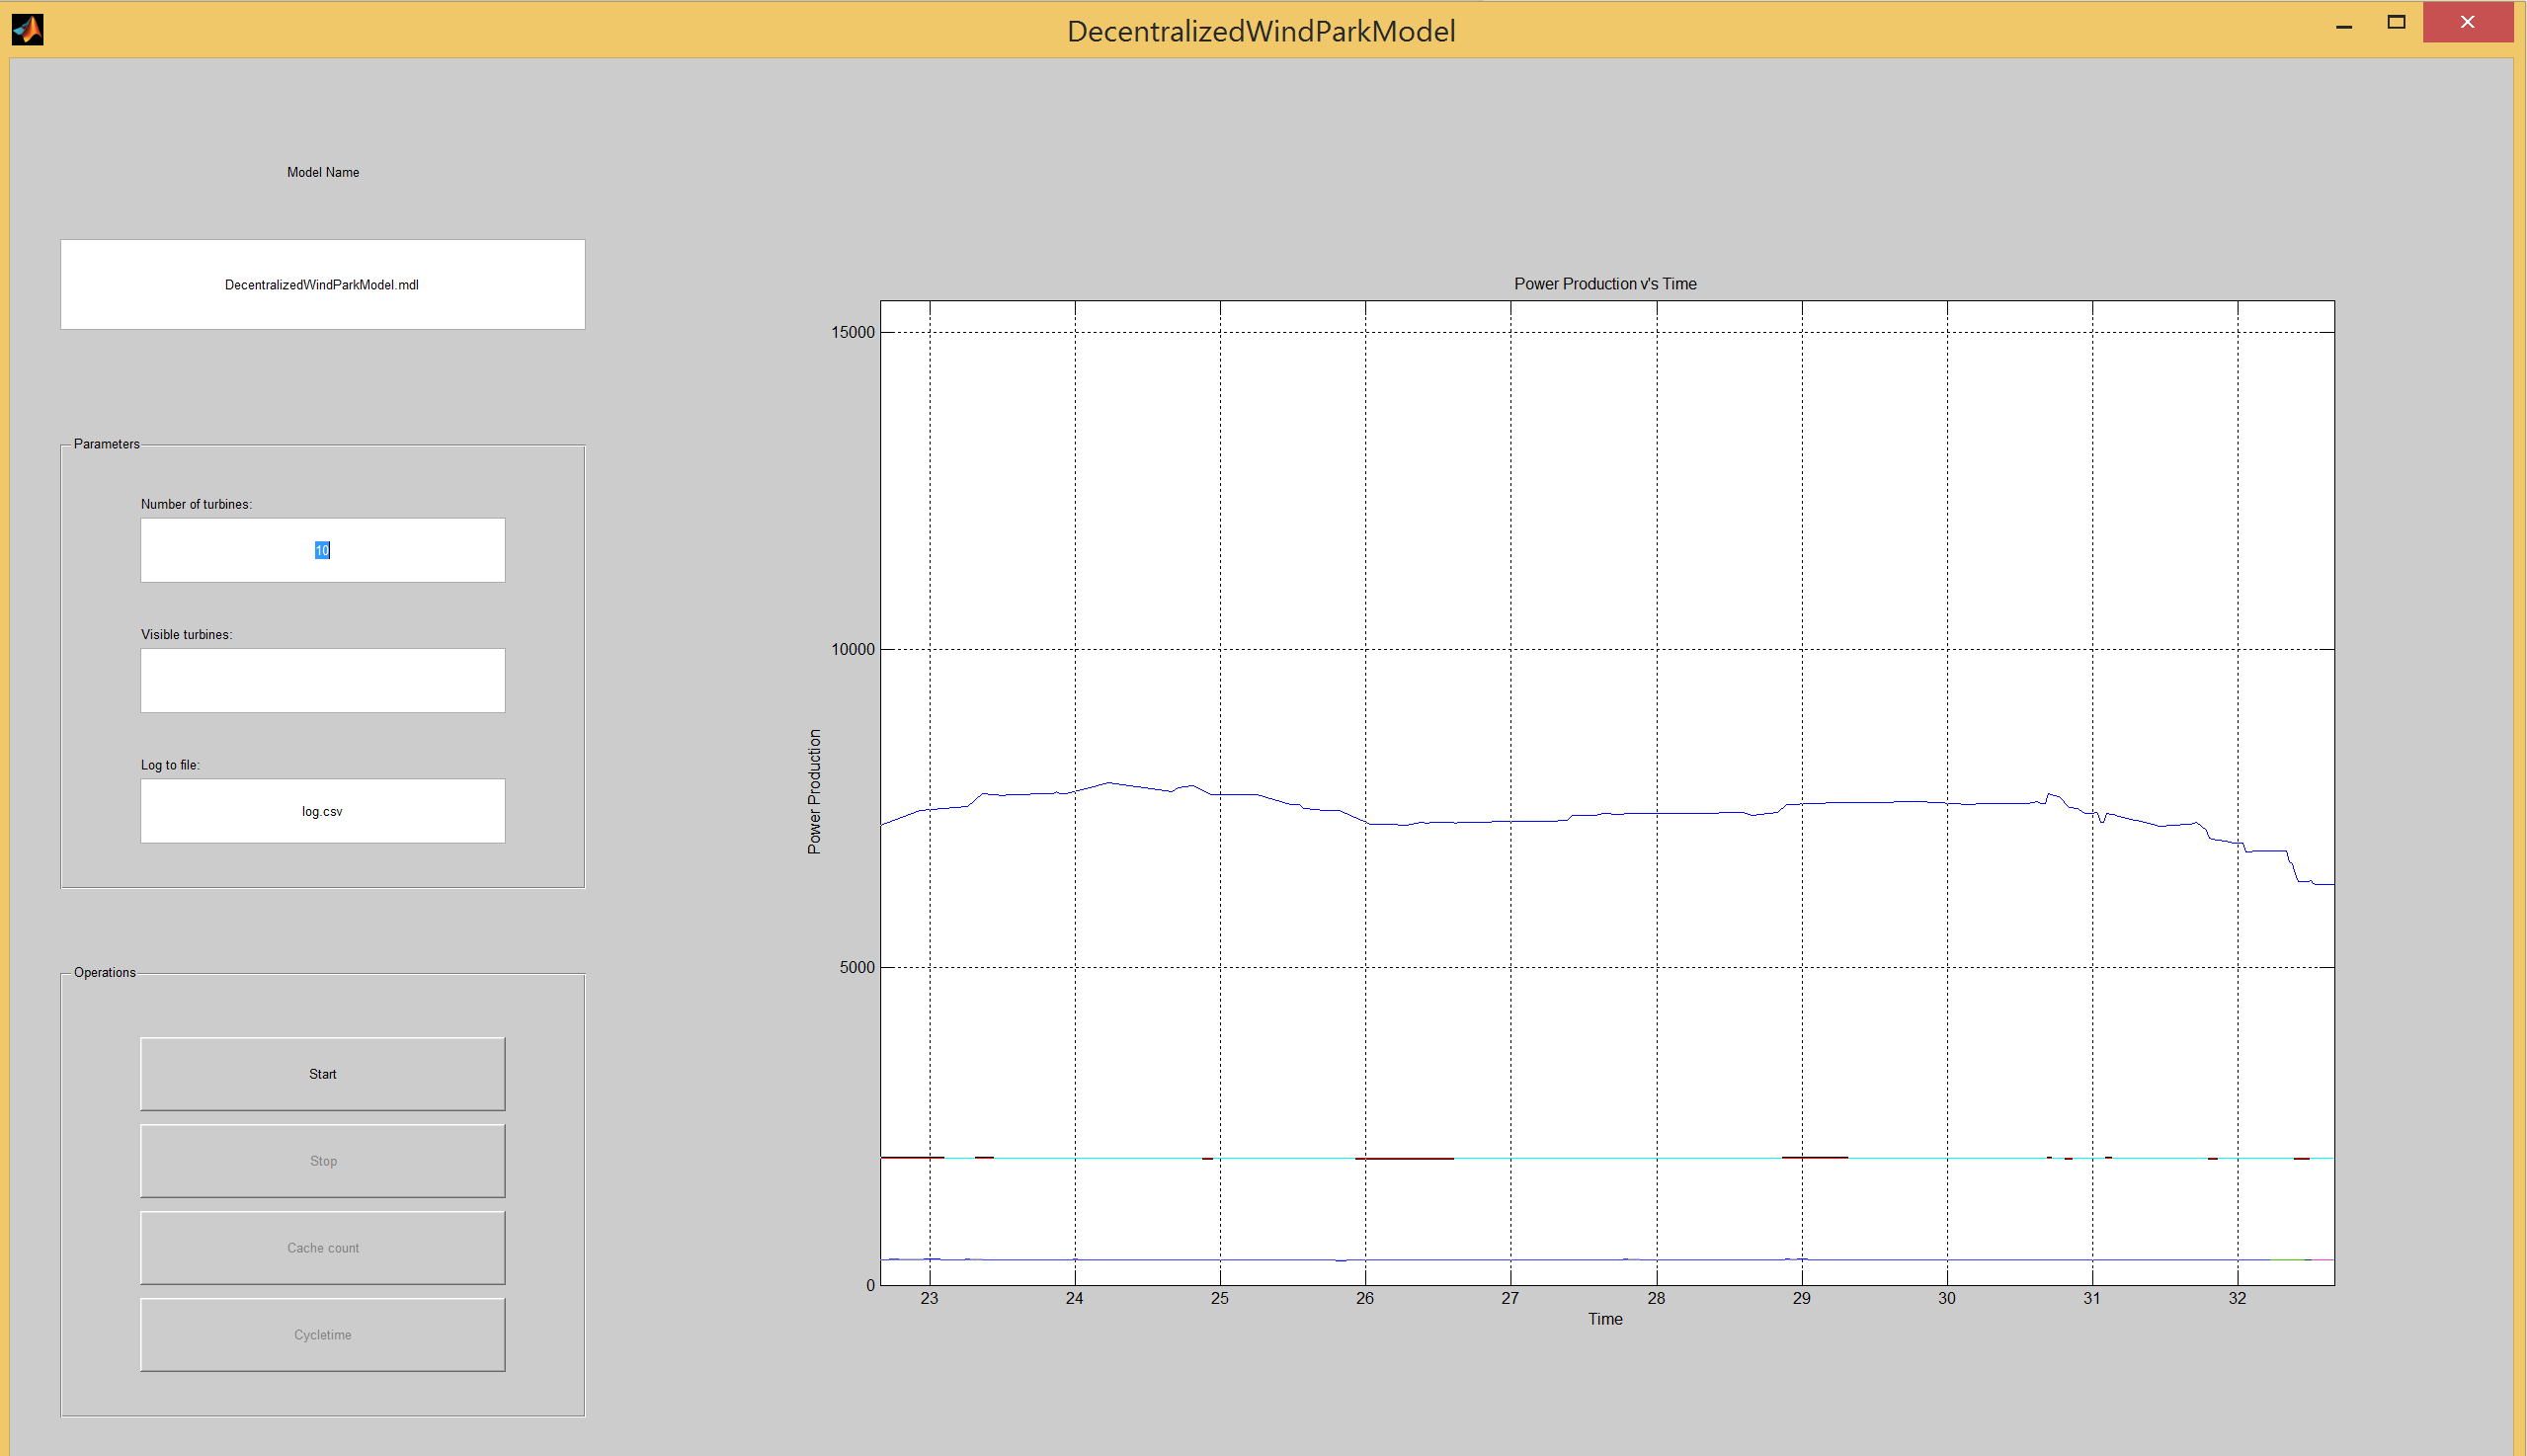
\includegraphics[width=\resultsFigureWidthScale\textwidth]{gui.png} 
	\captionsetup{format=plain,font=footnotesize,labelfont={bf,defaultCapFont},labelsep=quad,singlelinecheck=no}
	\caption[Graphical interface running 10 turbines]{
		\label{fig:graphicalInterface} 
		\footnotesize{%
			Graphical interface running 10 turbines.
		}
	}
\end{figure}

Presented in \cref{fig:graphicalInterface} is a screenshot of the graphical interface made with DDS Blockset for Simulink (described in section \cref{sec:graphicalInterface}). The x-axis show Time in seconds and the y-axis show kW production. The screenshot is taken while the decentralized solution runs 10 turbines.
The global setpoint for power production is illustrated by the red line and is showing a value of just below 5000 kW. The global power production is illustrated by the black line also just below 5000 kW.
The blue line illustrates the maximum available power production for the wind farm which, during this experiment, was above 10000 kW. The lines at the bottom shows values of around 500 kW and they each represents the current power production of each turbine.

\subsection{Discussion}\label{feas:discussion}
The experiment performed to prove whether or not it is feasible to create a decentralized solution that is able to do power regulation, consists of a simple run of the prototype of the decentralized solution. The global setpoint and the global production line match and thus we conclude that we have a working prototype, that can regulate according to the global setpoint. Each turbine is expected to produce $globalSetpoint/nTurbines=5000kW/10=500kW$(see \cref{sec:calculateSetpoints} for detailed description of the regulation algorithm), which they do. The slight deviation (the deviation that makes each turbine produce close to 500kW and not exactly 500kW) is due to the regulation algorithm being inaccurate. For the purpose of this experiment, the fact that the regulation algorithm is inaccurate is acceptable since the regulation algorithm is black box and not the focus of this thesis.

As such it is hard to deduce from a screenshot that the decentralized solution is actually able to perform power regulation, but this experiment in correlation with the rest of the experiments performed in this chapter will show that the prototype is functioning.

In order to decentralize fully decentralize the current Siemens system, decentralization of the Wind Power Supervisor must also be covered. The purpose of the Wind Park Supervisor is to log data from every turbine within the farm and handle external communication. Thus the Wind Park Supervisor consists of two primary features: Data storage and aggregation and external communication. 

Decentralizing the data storage and aggregation onto the turbines requires a horizontally scalable distributed database, which can handle data aggregation. Distributing the database horizontally is important in order to handle datasets larger than the physical storage of one turbine and data aggregation is needed for the case where an external request requires data to be aggregated. To handle this MongoDB~\cite{mongodb} has been identified as the optimal component (as concluded in \cref{sec:databaseStorage} Data Storage). MongoDB supports Sharding for automatic horizontal partitioning of datasets and data aggregation. MongoDB has been chosen based on other parameters related to the problems \ref{PS:Q:Availability} and \cref{PS:Q:Performance}, however to answer the answer the \ref{PS:Q:Feasibility} problem, this functionality is sufficient. 

Handling external communication decentralized means, BLABLA \todo{KRAUSE} has been identified as the optimal component.

\clearpage
\section{\ref{PS:Q:Availability}}

\textit{Can we create a solution where removing one or more nodes from the system at runtime does not cause system failure?}\newline\newline

\noindent To answer whether or not a fully decentralized current Siemens system can handle removing one or more nodes at runtime, the discussion section of this experiment also contains a discussion with regards to the components analyzed in \cref{cha:stateOfTheArt}: \nameref{cha:stateOfTheArt}.\todo{Why the chapter name ref?}

\subsection{Experiments}
The \ref{PS:Q:Availability} problem address if the proposed decentralized solution is able to continue its functions even though nodes are interrupted and removed from the system at runtime.
The proposed decentralized solution should be able to continue maintaining the global setpoint of the wind farm even if some turbines become unavailable, assuming that the needed production capacity is available.

The below experiment is repeated with $N = 1, 5, 10, 15$ failing turbines of 30 running turbines.
%
The experiment has the following procedure:
\begin{enumerate}
	\item Start the system with 30 turbines.
	\item Make sure the system is stable.
	\item Kill N nodes.
\end{enumerate}

Did the system adjust the setpoints for all turbines to maintain the global setpoint?

\subsection{Results}
\label{sec:res:availability}
The plots in \cref{fig:exp:availability_kill15,fig:exp:availability_kill10,fig:exp:availability_kill5,fig:exp:availability_kill1} show how the decentralized solution reacts when killing 1, 5, 10 and 15 turbines. The figures are Matlab screen shots from the graphical interface presented in \cref{sec:graphicalInterface}. The x-axis show time in seconds and the y-axis show kW production. The global setpoint is set to 20,000~kW instead of 2000~kW for the experiment with 1 failing turbine is removed (\cref{fig:exp:availability_kill1}). The global setpoint value for this experiment has been set this high to provide a better visual representation for the case where 1 turbine has crashed. 
% (a change of $globalSetpoint/nTurbines=2,000kW/30=66,6kW$ is harder to see than change of $20,000kW/30=666,6kW$). 
For the remainder of the cases (meaning where 5, 10 and 15 turbines are crashed), the global setpoint is set to 2000~kW.
The turbines are all running with a cycle time of 20 ms throughout this experiment.

\clearpage
\Cref{fig:exp:availability_kill1} shows an increase of production pr. turbine by approximately 20 kW pr. remaining turbines, after a single turbine is crashed. A global setpoint of 20,000kW was set for this test.

\begin{figure} [!h]
	\centering
	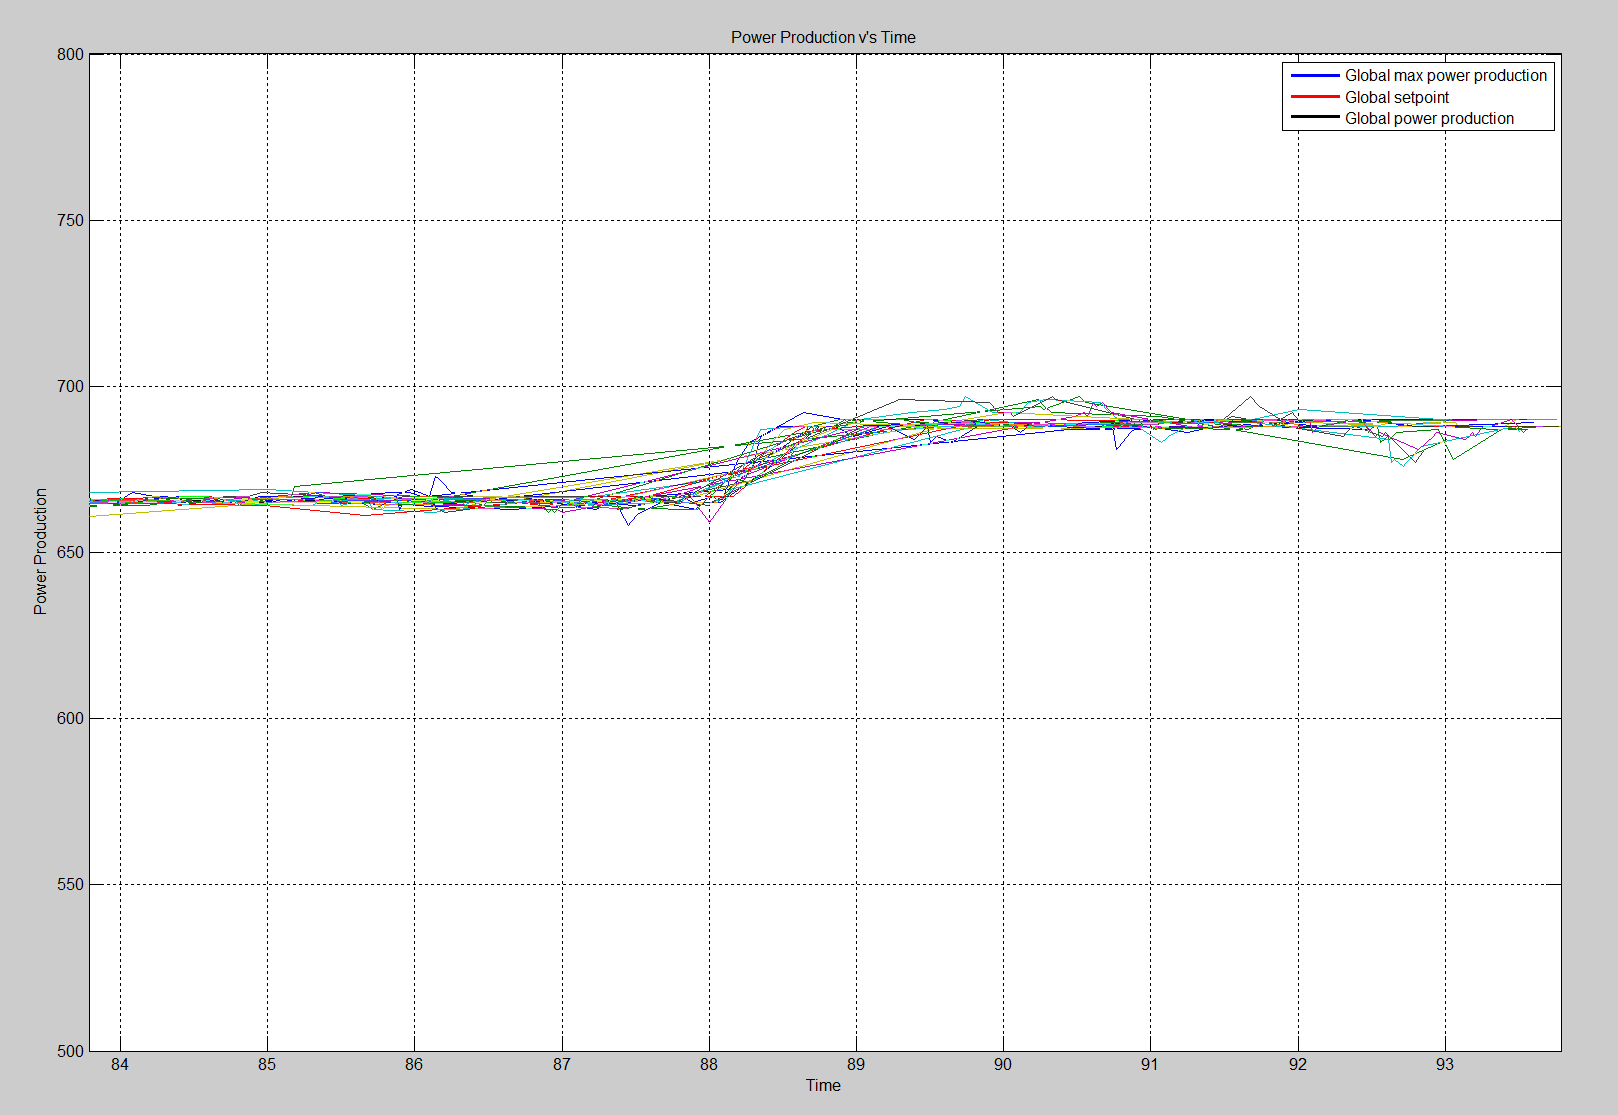
\includegraphics[width=\resultsFigureWidthScale\textwidth]{figures/Results/availabilitytest30-29_setpoint_20000.PNG}
	\caption{Availability test kill 1 out of 30 turbines}
	\label{fig:exp:availability_kill1}
\end{figure}

\Cref{fig:exp:availability_kill5} shows an increase of production pr. turbine by approximately 15 kW pr. remaining turbines, after 5 turbines are crashed. A global setpoint of of 2000kW was set for this test.

\begin{figure} [!h]
	\centering
	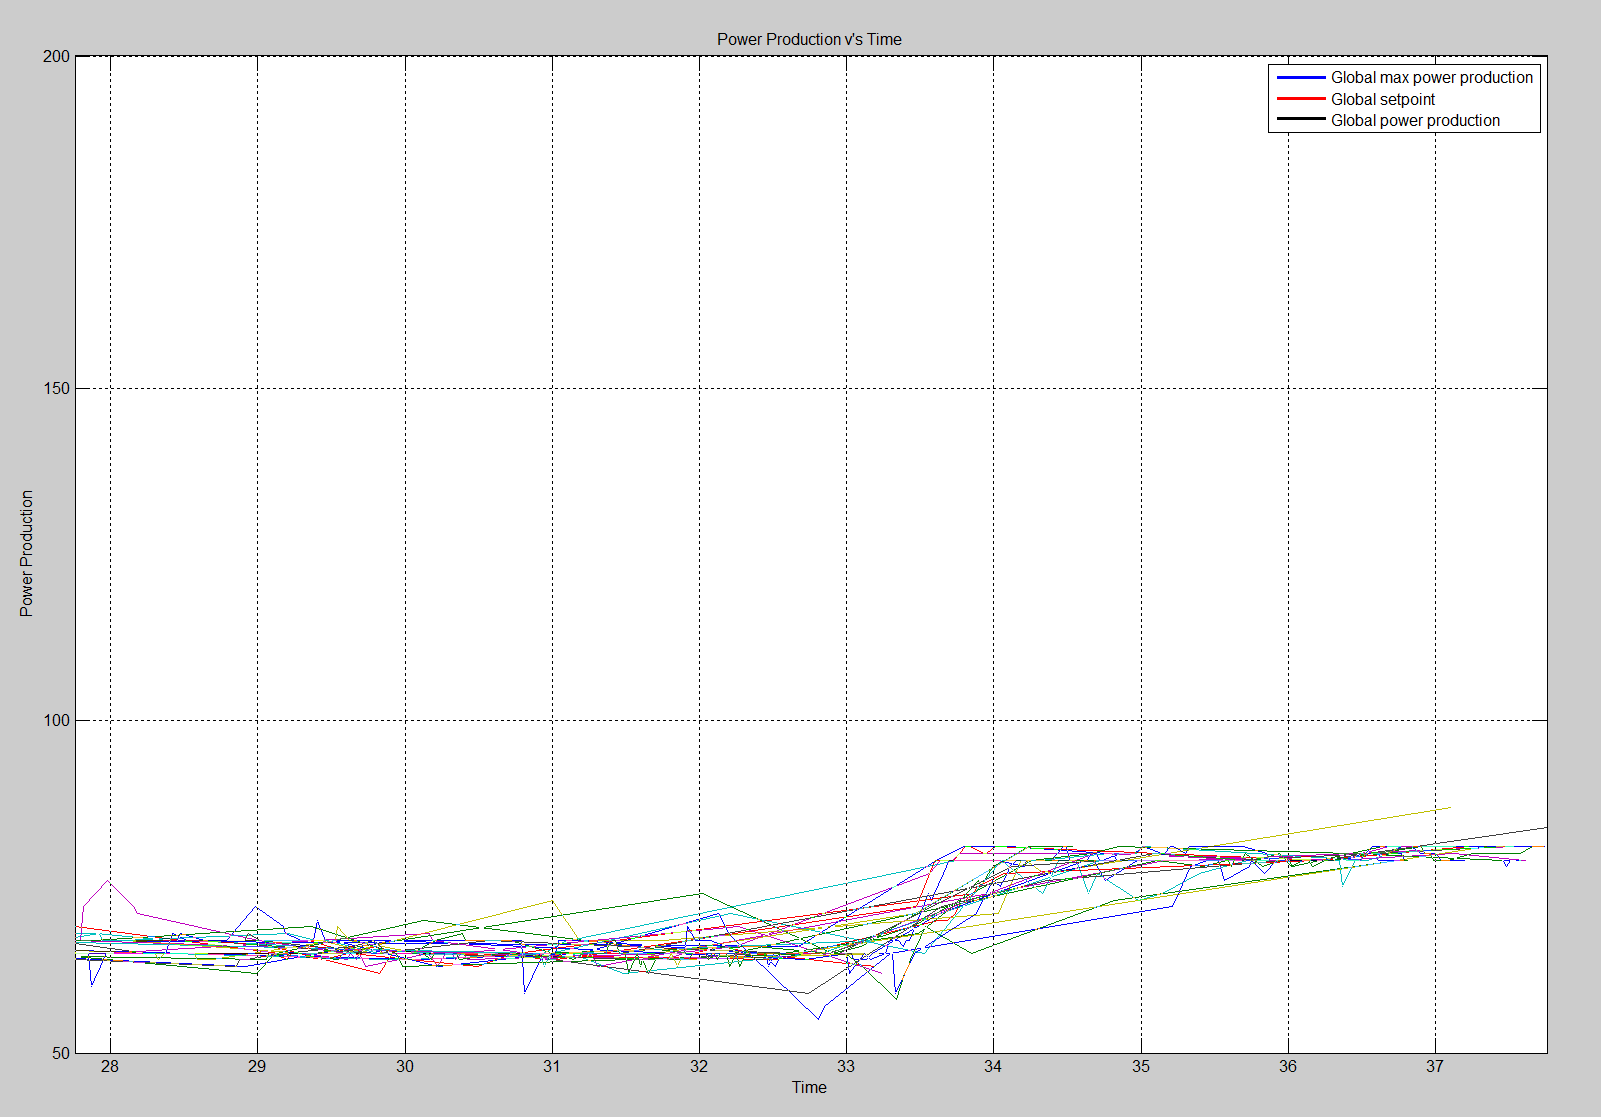
\includegraphics[width=\resultsFigureWidthScale\textwidth]{figures/Results/availabilitytest30-25_setpoint_2000.PNG}
	\caption{Availability test kill 5 out of 30 turbines}
	\label{fig:exp:availability_kill5}
\end{figure}

\FloatBarrier
\Cref{fig:exp:availability_kill10} shows an increase of production pr. turbine by approximately 30 kW pr. remaining turbines, after 10 turbines are crashed. A global setpoint of of 2000kW was set for this test.

\begin{figure}[!h]
	\centering
	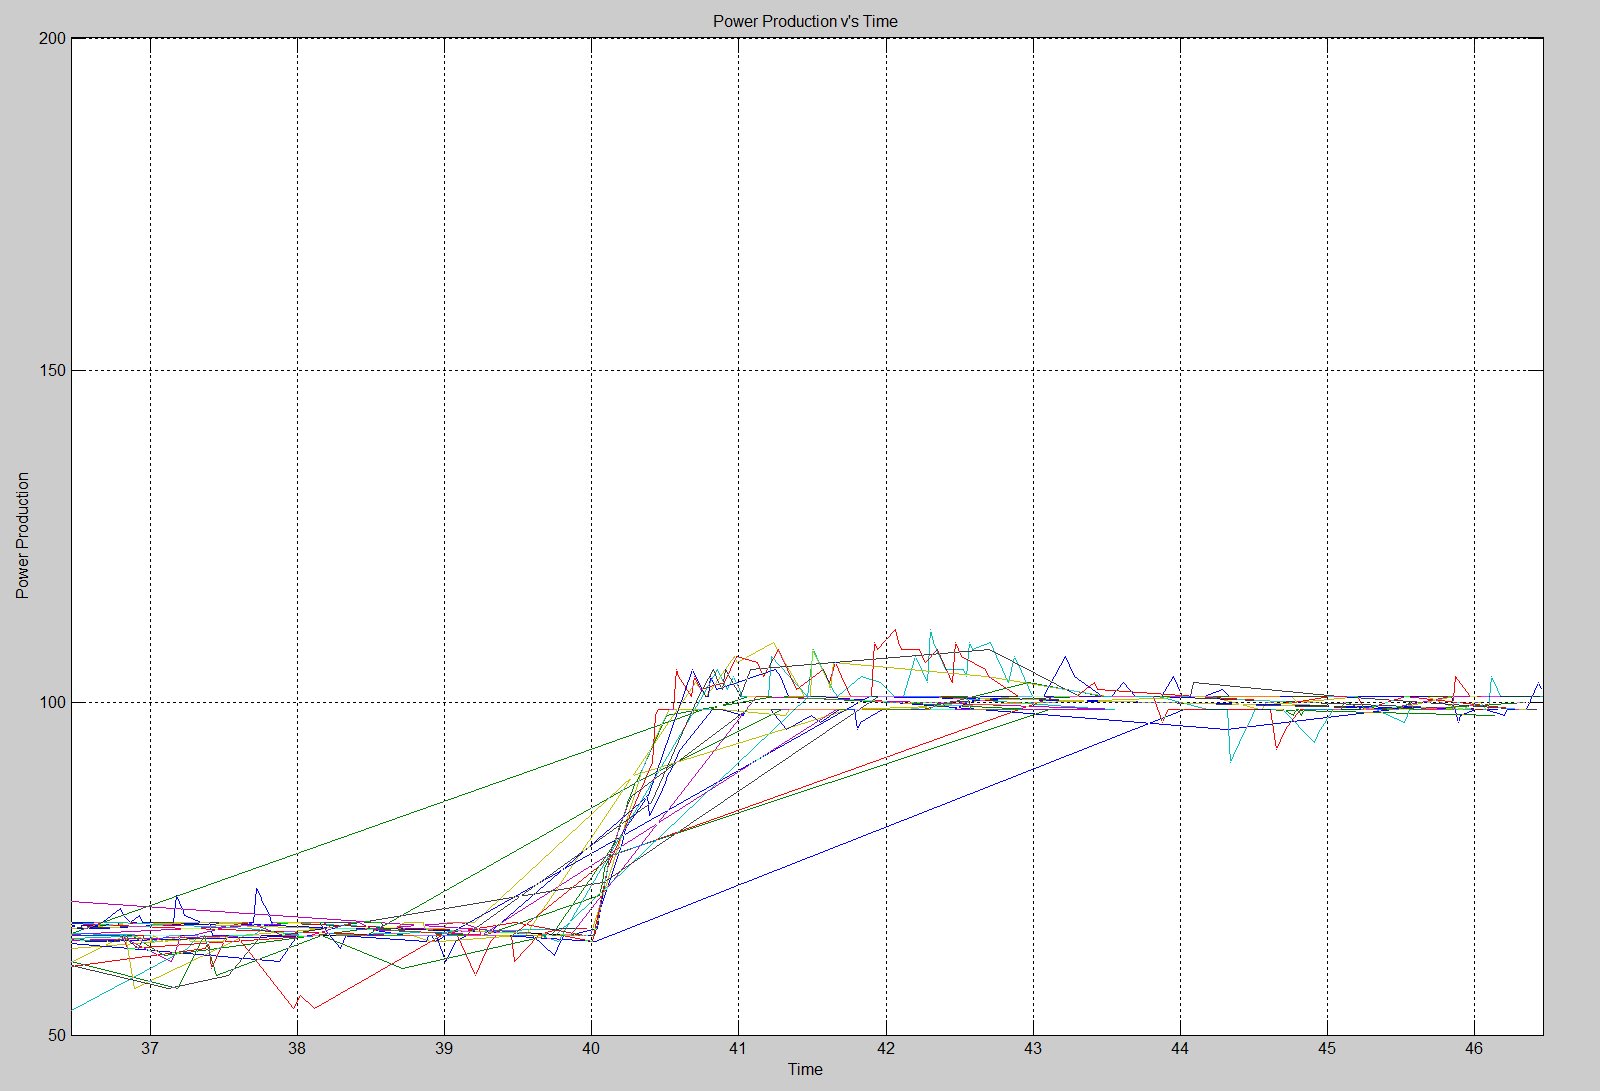
\includegraphics[width=\resultsFigureWidthScale\textwidth]{figures/Results/availabilitytest30-20_setpoint_2000.PNG}
	\caption{Availability test kill 10 out of 30 turbines}
	\label{fig:exp:availability_kill10}
\end{figure}

\FloatBarrier
\Cref{fig:exp:availability_kill15} shows an increase of production pr. turbine by approximately 60 kW pr. remaining turbines, after 15 turbines are crashed. A global setpoint of of 2000kW was set for this test.

\begin{figure}[!h]
	\centering
	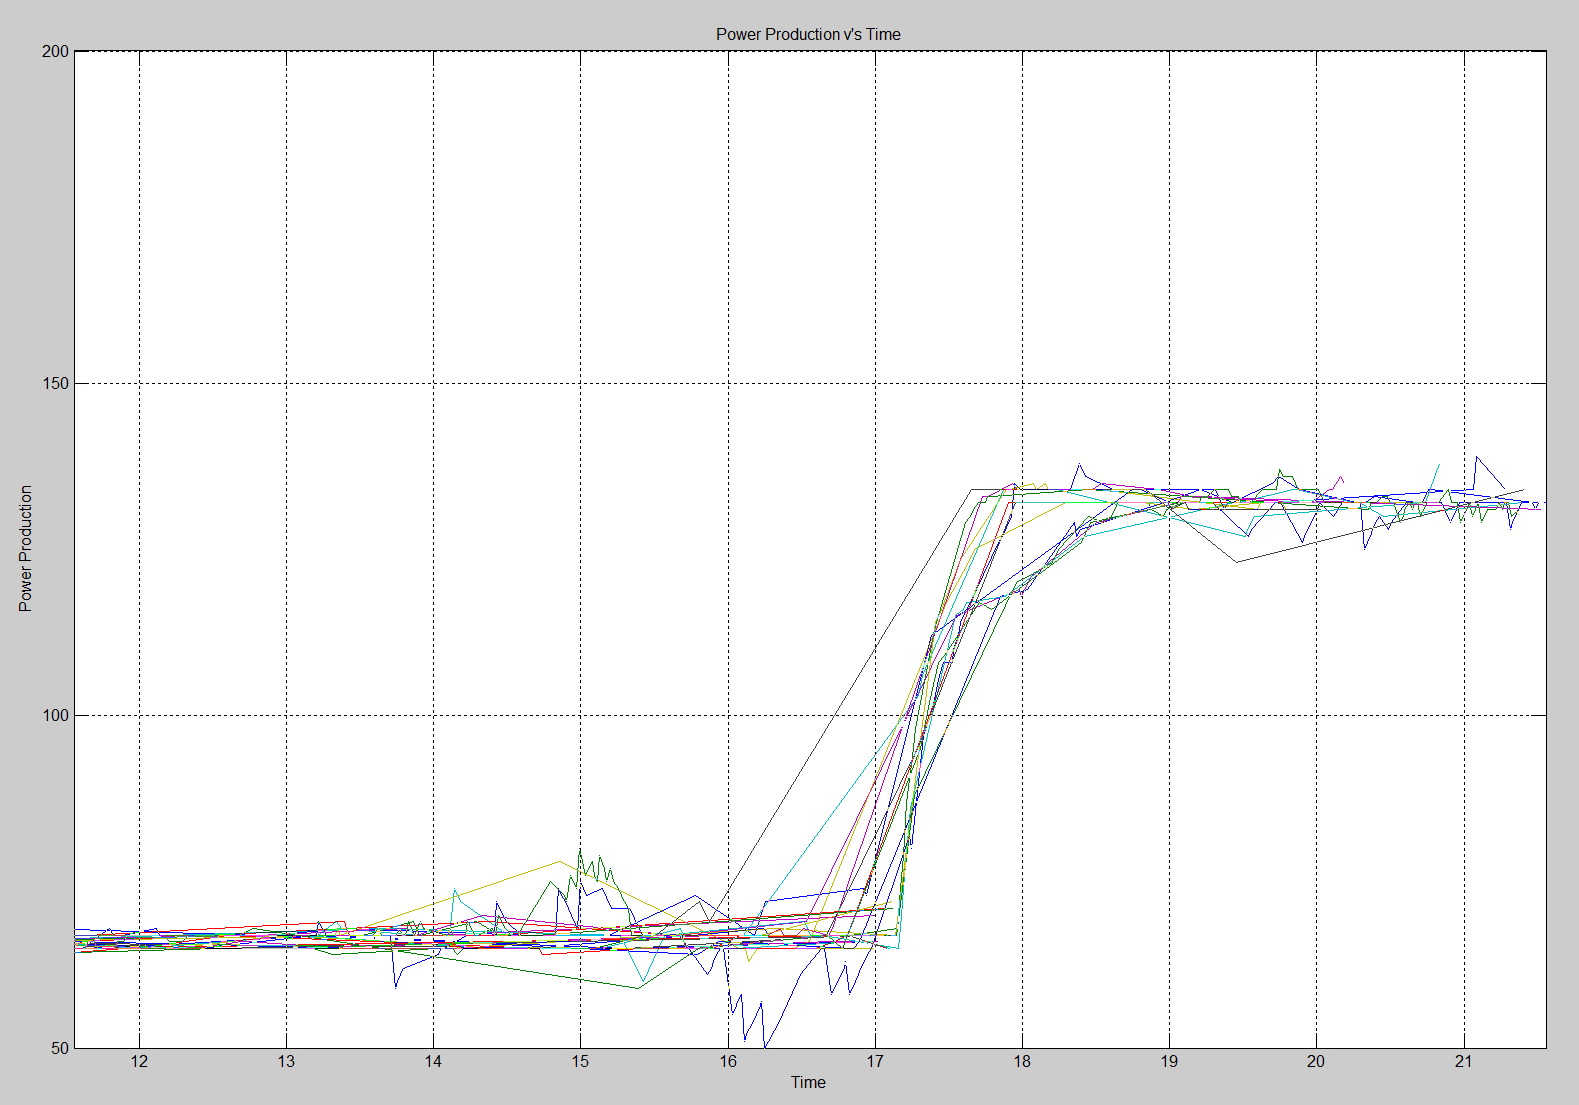
\includegraphics[width=\resultsFigureWidthScale\textwidth]{figures/Results/availabilitytest30-15_setpoint_2000.PNG}
	\caption{Availability test kill 15 out of 30 turbines}
	\label{fig:exp:availability_kill15}
\end{figure}

\FloatBarrier

The 'glitches' in the figures, where the plots shows several seconds between some of the data points, are properly caused by the eventhandler in Matlab handling events from DDS Blockset for Simulink (described in \cref{sec:graphicalInterface}). The eventhandler appears to be neglecting some of the events caused by the publication of turbine states, thus resulting in several seconds time interval between two data points. For the purpose of this experiment we are able to clearly see that it does the regulation, however the time frame is inaccurate.
\todo[inline]{Forklar udfra tråd problemmer istedet for at events bare ikke bliver sent afsted, samme gælder availability GUI afsnittet.}

\subsection{Discussion}
One of the main challenges of highly available is to continue operation in the event of node crashes or loss. As presented in  \cref{fig:exp:availability_kill15,fig:exp:availability_kill10,fig:exp:availability_kill5,fig:exp:availability_kill1} the decentralized solution can handle the loss of turbines. A turbine is considered offline if it does not publish any new data to any other turbines within a 150 ms timespan, defined by the Lifespan QoS parameter of the DataWriter described in \cref{sec:decen:ddsconf}.
This upper limit of 150 ms is chosen because 150 ms is the upper limit of the regulation cycle time in the current Siemens system.
% % % I am HERE Krause
After a turbine crash has been detected the remaining turbines in the wind farm will share the load of the now missing turbines, in order to restore the global power production to the global setpoint.

%The following turbine production increase formula is based on the regulation algorithm definition explained in \cref{sec:calculateSetpoints}.
Let k = the number of turbines crashed, p = production of the crashed turbine, and n = number of remaining turbines. The expected increase of production pr. turbine when k turbines have crashed, is denoted as: 
$$Production~increase~per~turbine = \frac{\sum\limits_{i=1}^k(p)}{n}$$

Thus the expected production increase for the case where a single turbine is crashed (\cref{fig:exp:availability_kill1}) is: $$\frac{\sum\limits_{i=1}^1(666,6kW)}{29}\approx23kW$$

Hence for the rest of the cases (note that the global setpoint for these cases are 2000kW, thus the production of each turbine is 66,6 kW as apposed to 666,6 kW for the case where one turbine was crashed):
\newline\newline
\noindent5 turbines crashed (\cref{fig:exp:availability_kill5}) $$\frac{\sum\limits_{i=1}^5(66,6kW)}{25}\approx13kW$$

\noindent10 turbines crashed (\cref{fig:exp:availability_kill10}) $$\frac{\sum\limits_{i=1}^{10}(66,6kW)}{20}\approx33kW$$

\noindent15 turbines crashed (\cref{fig:exp:availability_kill15}) $$\frac{\sum\limits_{i=1}^{15}(66,6kW)}{15}\approx67kW$$

These expected values matches the increased productions shown in \cref{fig:exp:availability_kill5,fig:exp:availability_kill10,fig:exp:availability_kill15}. The glitches \todo{Anden brug af glitches} in the figures are caused by the simulated turbine data and is therefore accepted for the purpose of this experiment. Thus we conclude that the remaining turbines share the extra load between themselves and power production continues after turbine crashes.
This means removing one or multiple turbines from the system does not impede the regulation of the wind farm.

%The time it takes the decentralized solution to detect a turbine loss and recover power production is dependent on the following parameters:
%
%\begin{itemize}
%	\item Time of turbine loss detection, which is defined by the History QoS to 150 ms, $I$.
%	\item Time between regulation cycles, in the test cases presented in \cref{sec:res:availability} the time is set to 20 ms, $S$.
%	\item Time of calulation of a new setpoint, $C$.
%	\item Time for the turbine to regulate power production according to the new setpoint. In the turbines this process is simulated with a simple regulation that may take several regulation cycles to complete $R$.
%\end{itemize}
%
%Thus the time for recovery of the power production when a turbine failure occurs can be calculated as $T = I + S + C + R$ which translates to $150 ms + 20 ms + C + R = 170 + C + R ms$. This time can be reduced by lowering the time it takes to detect a turbine is offline which increases the likelihood of detecting a delayed turbine as offline, or by lowering the time between regulation cycles which increases the likelihood of cache reads.

The time it takes for the turbines to regulate according to crashed turbines are of course an important factor.
\todo{Expalin why}
However since we are using an arbitrary regulation algorithm and turbine simulations, we cannot conclude anything with regards to this subject.

% The only thing we can conclude is that the turbines regulate according to multiple crashed turbines relatively fast, meaning that the time it takes for the turbines to regulate according to one or more crashes happens within an acceptable timeframe of 1 to 4 seconds. 

When it comes to availability for the a potential decentralized wind farm, handling the communication for the regulation algorithm run by the Park Pilot is only one part of the picture. Availability for the decentralized Wind Park Supervisor, which handles external communication and data storage and aggregation, must also be addressed. 

To ensure available data storage, the problem of data loss when a turbine is unresponsive must be addressed. A turbine has several control and measurement points which are continually logged to a local data store. Should a turbine break down, the local data may be destroyed with the turbine. This sets special requirements to the component handling data storage. In \cref{sec:databaseStorage} the requirements to the data storage component is described and MongoDB was identified as the best choice to solve the availability problem related to data storage. MongoDB is capable of replication of data between turbines, such that data is still available should a turbine crash occur. As well as replication MongoDB provides sharding of a database, which enables a global database to be stored across multiple nodes. Replication and sharding can be combined such that no single node contains all global data. This is needed to prevent single point of failures. 

Sharding is needed in order to make the database scale horizontally. Thus in order to make a system where removing nodes from the system does not cause system failure, replication of each shard is needed. However, replication of shards only solve the problem to some extent, since removing all replicated copies of a single shard renders the shard unavailable, thus rendering a part of the database unavailable. To prevent this from happening, an appropriate amount of turbines must be allocated per shard. This to heighten the availability of the wind farm, increasing the number of turbines per shard, however this also increases the amount of data storage used for the database, since it causes duplicated data. Thus increasing availability of the system is at the cost of data storage used per turbine.

Making the decentralized solution robust and able to handle the loss of turbines with regards to internal communication, regulation of power production, external communication and data storage increases the overall availability of the wind farm. %With MongoDB chosen for data storage and BLABLA chosen for resource management, we conclude availability for the case where removing a few amount of nodes does not cause system failure is definitely feasible. Increasing the number of turbine crashes the system needs to be able to handle increases the disk storage needed on each turbine.

To handle communication with the outside world we use a load balancer as a single external entry point, 
however it must be prevented that it becomes a single point of failure.
To prevent this we are using a load balancer with automatic fail over, in section \cref{cha:resourceManagement} such a system described.
It continuously keep the active connections information synchronized between active and backup nodes and uses heartbeat monitoring to detect a node crash.
The load balancer setup helps solve the \ref{PS:Q:Availability} problem.

\clearpage

\section{\ref{PS:Q:Performance}}

\textit{Can we create a solution that scales such that the number of turbines does not impact the regulation cycle time?}

\subsection{Experimenit}
\label{sec:Exper:perfom}

%Scalability is by Bondi\cite{Bondi:2000:CSI:350391.350432} defined as \textit{the systems ability to accommodate an increasing number of elements or objects, to process growing volumes of work gracefully, and/or to be susceptible to enlargement}.

The \ref{PS:Q:Performance} question asks if the proposed decentralized solution is able to keep a constant regulation cycle time independent from the number of turbines. This problem operates in a 3-dimensional space with cycle time (ms), number of cache reads and number of turbines as parameters. To study the correlation between the parameters, we isolate two parameters by making the third constant.

Thus to fully address \ref{PS:Q:Performance} this experiment has been divided into two experiments:
 
\begin{description}
	\item[Experiment 1] aims to investigate the anti-correlation between the implemented sleep time of the regulation cycle and the number of cache reads for the decentralized system. This is relevant because changing the sleep time is expected to impact the number of cache reads, since an increase in sleep time increases the time Connext has to overwrite received states, thus decreasing the number of cache reads (as explained in \cref{sec:cachereads}: Cache reads). Thus the constant for this is experiment is the number of turbines.
	\item[Experiment 2] aims to investigate the impact on the regulation cycle time and the number of cache reads when increasing the number of turbines in the decentralized solution, and thus answer the \ref{PS:Q:Performance} problem. The constant for this experiment is the sleep time.
\end{description}


\subsection{Experiment 1: How sleep time impacts the regulation cycle time and the number of cache reads}
\label{subsec:Exper:perfom:1}
The purpose of this experiment is to show how the sleep time affects the number of cache reads and the regulation cycle time for the decentralized solution (see \cref{sec:cachereads} for cache reads description).  
The experiment is performed with cycle time t=\testCycletimeNumbers.  

The following procedure is used each time the experiment is performed:
\begin{enumerate}
	\item Start the system with a cycle time of t ms and 21 turbines.
	\item Make sure the system is stable.
	\item Start logging the regulation cycle time and the number of cache reads.
	\item Stop logging when 1000 data points are reached.
\end{enumerate}

\subsection{Experiment 2: How the number of turbines impacts the regulation cycle time and the number of cache reads}
\label{subsec:Exper:perfom:2}
The purpose of this experiment is to answer the \ref{PS:Q:Performance} problem, by showing how the number of turbines affects the regulation cycle time for the decentralized solution. To complete the picture we also investigate how the number of turbines affects the cache reads, since an expected side effect of increasing the number of turbines also increases the number of cache reads as described in \cref{sec:cachereads}.

The experiments are performed with n=\testTurbineNumbers ~turbines. The sleep time is set to 20 ms and is constant for this experiment.

The test system is expected to be running only one instance in a real life implementation, therefore the machine logging the data will only run one instance and the supporting machines will run the rest generating system load.

The following procedure is used each time the experiment is performed:
\begin{enumerate}
	\item Start the system with N turbines.
	\item Make sure the system is stable.
	\item Start logging the reported regulation run time and the number of cache reads.
	\item Stop logging when 1000 data points are reached.
\end{enumerate}


\subsection{Results}

\label{sec:exp:performance}
The cycle regulation time is defined as the difference between the receive timestamp of the oldest turbine state(tOldestState) received and the timestamp sampled right after, a new turbine state has been sent (tSent) (as illustrated on \cref{fig:timingDecentral}):

$$regulation~cycle~time=tSent-tOldestState$$

\begin{figure}[b]
	

{ %The brackets issolate the enviroment

\makeatletter
\ifcsname c@wavenum\endcsname %Only create one counter
\else
	\newcounter{wavenum}
\fi
\makeatother

\newcommand*{\bitvector}[3]{
  \draw[fill=#3] (t_cur) -- ++( .1, .3) -- ++(#2-.2,0) -- ++(.1, -.3)
                         -- ++(-.1,-.3) -- ++(.2-#2,0) -- cycle;
  \path (t_cur) -- node[anchor=mid](textNode) {#1} ++(#2,0) node[time] (t_cur) {};
}

% \known{val}{length}
\newcommand*{\known}[2]{
    \bitvector{#1}{#2}{white}
}

% \unknown{length}
\newcommand*{\unknown}[2]{
    \bitvector{#1}{#2}{black!20}
}

% \nextwave{name}
\newcommand{\nextwave}[1]{
  %\path (0,\value{wavenum}) node[left] {#1} node[time] (t_cur) {};
  \path (0,\value{wavenum}) node[time] (t_cur) {};
  \addtocounter{wavenum}{-1}
}

%\newcommand{\timeSpanLabel}{
%	\node (CycleTimeLabel) [rectangle, above = 0.25cm of textNode, inner sep=10pt] {CycleTime};	  
%}

\newcommand{\timeSpanLabel}{
	\node (CycleTimeLabel) [rectangle, above = 1.02cm of t_cur, inner sep=0pt] {Regulation cycle time};
}

\newcommand{\timeSpanA}{
	\node (t_timeSpanA) [point, above = 0 of t_cur] {};	  
}

\newcommand{\timeSpanB}{
	\node (t_timeSpanB) [point, above =0 of t_cur] {};
	
	\graph[use existing nodes]{
		t_timeSpanA --[time span=1cm] CycleTimeLabel;
		CycleTimeLabel.south --[time span=-0.24cm] t_timeSpanB;
	}; 
	
}

%%% End of timing.sty

\begin{tikzpicture}[
	point/.style={inner sep=0pt}, %circle,minimum size=2pt,fill=red},
	draw=black, 
	yscale=.8,
	xscale=1,
	hv path/.style={to path={-| (\tikztotarget)}},
	vh path/.style={to path={|- (\tikztotarget)}},
	skip loop v/.style={to path={-- ++(#1,0) |- (\tikztotarget)}},		
	skip loop h/.style={to path={-- ++(0,#1) -| (\tikztotarget)}},
	time span/.style={to path={-- ++(0,#1) -| (\tikztotarget)}},
	graphs/every graph/.style={edges=rounded corners}	
]
	
\tikzstyle{time}=[coordinate]
\setlength{\unitlength}{1cm}
\setcounter{wavenum}{0}

	\nextwave{} \timeSpanA \unknown{readStates}{3} \unknown{calculate}{3} \timeSpanLabel \unknown{setSetpoint}{3} \unknown{sendState}{3} \timeSpanB \known{wait}{2}
	\nextwave{} \known{reciveStates}{14}
\end{tikzpicture}
}

	\caption{Decentralized regulation time}
	\label{fig:timingDecentral}
\end{figure}

The timestamp of the oldest turbine state is used to include network traffic in the regulation cycle time, as opposed to just sampling the time locally.

We use the following box plot type (for \cref{fig:exp:decen:sleep} and \cref{fig:exp:decen:turbines}): The central mark is the median, the edges of the box are the 25th and 75th percentiles, the whiskers extend to the most extreme data points not considered outliers, and outliers are plotted individually. The whisker length is denoted as 1.5 IQR. 

The red line plots the medians.

\subsubsection{\nameref{subsec:Exper:perfom:1}}

\begin{figure}[h!]
	\centering
	\begin{tikzpicture}
\begin{axis}
[
width=\resultsFigureWidthScale\textwidth,
axis y line*=left,
xlabel=Sleeptime (ms),
ylabel=Regulation cycle time (ms),
ymin = 0,
xtick={1, 2, 3, 4, 5, 6, 7, 8, 9},
xticklabels={10, 15, 20, 25, 30, 35, 40, 45, 50},
boxplot/draw direction=y
]

%% /home/stefan/work/TestResults/Test6_Decentralized_12-7-2014_1327/nCycleTime/DecentralizedLog1.csv
\buildBoxPlot{10.578002}{15.286001}{9.942}{148.911}{0.415002}

%% /home/stefan/work/TestResults/Test6_Decentralized_12-7-2014_1327/nCycleTime/DecentralizedLog2.csv
\buildBoxPlot{15.026002}{15.383002}{14.312002}{26.729001}{1.379}

%% /home/stefan/work/TestResults/Test6_Decentralized_12-7-2014_1327/nCycleTime/DecentralizedLog3.csv
\buildBoxPlot{19.926}{20.380001}{18.979001}{29.932002}{0.435}

%% /home/stefan/work/TestResults/Test6_Decentralized_12-7-2014_1327/nCycleTime/DecentralizedLog4.csv
\buildBoxPlot{25.079001}{25.322}{24.637001}{32.794001}{12.225002}

%% /home/stefan/work/TestResults/Test6_Decentralized_12-7-2014_1327/nCycleTime/DecentralizedLog5.csv
\buildBoxPlot{30.099}{30.363}{29.565001}{42.436}{4.466}

%% /home/stefan/work/TestResults/Test6_Decentralized_12-7-2014_1327/nCycleTime/DecentralizedLog6.csv
\buildBoxPlot{35.153001}{35.328002}{34.853001}{45.836001}{10.347}

%% /home/stefan/work/TestResults/Test6_Decentralized_12-7-2014_1327/nCycleTime/DecentralizedLog7.csv
\buildBoxPlot{40.157001}{40.434001}{39.626}{58.338001}{6.398001}

%% /home/stefan/work/TestResults/Test6_Decentralized_12-7-2014_1327/nCycleTime/DecentralizedLog8.csv
\buildBoxPlot{45.185}{45.330001}{44.928002}{50.089}{29.313}

%% /home/stefan/work/TestResults/Test6_Decentralized_12-7-2014_1327/nCycleTime/DecentralizedLog9.csv
\buildBoxPlot{49.958002}{50.391001}{49.019}{64.611002}{4.846}


\addplot[thick, red!70] coordinates {
	(1 ,10.578002)
	(2 ,15.026002)
	(3 ,19.926)
	(4 ,25.079001)
	(5 ,30.099)
	(6 ,35.153001)
	(7 ,40.157001)
	(8 ,45.185)
	(9 ,49.958002)
	
};

\end{axis}
\end{tikzpicture}

	\caption{Decentralized solution with variable wait time cycle time experiment}
	\label{fig:exp:decen:sleep}
\end{figure}

\Cref{fig:exp:decen:sleep} show that the regulation cycle times and wait times are linearly dependent on each other. The maximum value with wait time 10 is outside the boundaries of the plot but is calculated to 148.91 ms. The upper and lower quartile are close together the exception is the 10 ms wait time sample. The maximum being the 20 ms wait time having a difference of 1.401 ms between upper and lower quantile and the minimum being 45 ms wait time with a difference of 0.402 ms. The maximum values again with the exception of the 10 ms wait time sample follow the median values, the minimum values are able to reach low regulation cycle times much lower than the wait time used in the experiment.

\begin{figure}[h!]
	\centering
	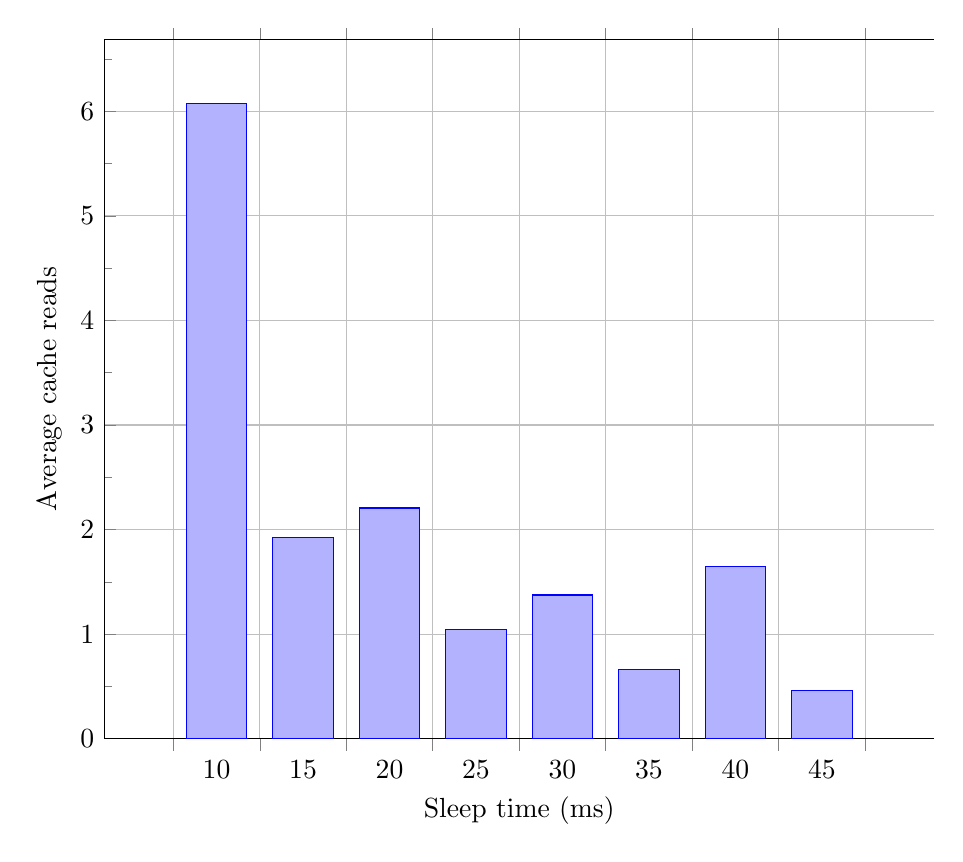
\begin{tikzpicture}
\begin{axis}
[
width=\resultsPlotWidthScale\textwidth,
axis y line*=left,
xlabel=Sleep time (ms),
ymin = 0,
%xmin = 0,
ylabel=Average cache reads,
%xtick={1, 2, 3, 4, 5, 6, 7, 8, 9},
%xticklabels={10, 15, 20, 25, 30, 35, 40, 45, 50},
%boxplot/draw direction=y,
%grid=both,
%ymajorgrids=true,
%yminorgrids=true,
ybar interval=0.7,
ymajorgrids=true,
%yminorgrids=true,
minor y tick num=1
%minor tick num=1
]
%\buildBoxPlot[black]{0}{0}{0}{0}{0}
%\buildBoxPlot[black]{0}{0}{0}{0}{0}
%\buildBoxPlot[black]{0}{0}{0}{0}{0}
%\buildBoxPlot[black]{0}{0}{0}{0}{0}
%\buildBoxPlot[black]{0}{0}{0}{0}{0}
%\buildBoxPlot[black]{0}{0}{0}{0}{0}
%\buildBoxPlot[black]{0}{0}{0}{0}{0}
%\buildBoxPlot[black]{0}{0}{0}{0}{0}
%\buildBoxPlot[black]{0}{0}{0}{0}{0}
\addplot coordinates {
	(10 ,6.076278918444858)
	(15 ,1.9250837336102817)
	(20 ,2.206446850393701)
	(25 ,1.044688862465319)
	(30 ,1.3747593094220163)
	(35 ,0.661782154722354)
	(40 ,1.6464805561590268)
	(45 ,0.46317152740208856)
	(50 ,1.858914282814271)
};

%matlab info
%     General model:
%     f(x) = (a/(x+b))+ c
%     Coefficients (with 95% confidence bounds):
%     a =       7.017  (-8.781, 22.82)
%     b =      -8.622  (-11.55, -5.697)
%     c =      0.9821  (0.01249, 1.952)
     
%\addplot[
%red,
%domain=10:50,
%samples=201,
%]
%{(7.017/(x-8.622))+ 0.9821};

\end{axis}
\end{tikzpicture}
	\caption{Decentralized solution with variable wait time cache reads experiment}
	\label{fig:exp:decen:sleep-cache}
\end{figure}

\Cref{fig:exp:decen:sleep-cache} show the average cache reads of the experiment.
A cache read only happens in the decentralized solution and is a consequence of the separation of receiving data in a separate thread.
The cache read happens if the wait time elapses before all turbine instances have responded with state information. The Number dos not include information of if the same turbine instance state has been read from cache multiple times.
The number of cache reads is declining. 
%, a fitted function of the plot has been put on top (red), the plot is in Matlab fitted against the function $\dfrac{a}{x + b} + c$.

\clearpage
\subsubsection{\nameref{subsec:Exper:perfom:2}}
The plots in this section relates to the second part of the \nameref{sec:Exper:perfom} experiment. In this graph the regulation cycle time is plotted against a variating number of turbines.

\begin{figure}[h!]
	\centering
	\begin{tikzpicture}
\begin{axis}
[
width=\textwidth,
axis y line*=left,
xlabel=Number of turbines,
ylabel=Regulation cycle time (ms),
ymin = 0,
xtick={1, 2, 3, 4, 5, 6, 7, 8, 9, 10, 11, 12, 13, 14, 15, 16, 17, 18, 19, 20},
xticklabels={5, 10, 15, 20, 25, 30, 35, 40, 45, 50, 55, 60, 65, 70, 75, 80, 85, 90, 95, 100},
boxplot/draw direction=y
]

%% /home/stefan/work/TestResults/Test5_Decentralized_success_12-4-2014_2100/nTurbines/DecentralizedLog0.csv
\buildBoxPlot{19.526002}{20.412002}{15.272001}{26.620001}{0.282}

%% /home/stefan/work/TestResults/Test5_Decentralized_success_12-4-2014_2100/nTurbines/DecentralizedLog1.csv
\buildBoxPlot{20.257002}{20.365001}{20.158001}{24.403002}{0.828002}

%% /home/stefan/work/TestResults/Test5_Decentralized_success_12-4-2014_2100/nTurbines/DecentralizedLog2.csv
\buildBoxPlot{20.221001}{20.311002}{20.126002}{24.641001}{3.778}

%% /home/stefan/work/TestResults/Test5_Decentralized_success_12-4-2014_2100/nTurbines/DecentralizedLog3.csv
\buildBoxPlot{20.203002}{20.321002}{20.066}{24.962}{0.246002}

%% /home/stefan/work/TestResults/Test5_Decentralized_success_12-4-2014_2100/nTurbines/DecentralizedLog4.csv
\buildBoxPlot{20.174001}{20.343}{19.946}{25.983002}{0.273002}

%% /home/stefan/work/TestResults/Test5_Decentralized_success_12-4-2014_2100/nTurbines/DecentralizedLog5.csv
\buildBoxPlot{20.190001}{20.286002}{20.051}{24.771001}{10.959001}

%% /home/stefan/work/TestResults/Test5_Decentralized_success_12-4-2014_2100/nTurbines/DecentralizedLog6.csv
\buildBoxPlot{20.079}{20.391001}{19.563001}{27.503001}{0.371002}

%% /home/stefan/work/TestResults/Test5_Decentralized_success_12-4-2014_2100/nTurbines/DecentralizedLog7.csv
\buildBoxPlot{20.176}{20.303001}{19.965}{30.63}{9.225}

%% /home/stefan/work/TestResults/Test5_Decentralized_success_12-4-2014_2100/nTurbines/DecentralizedLog8.csv
\buildBoxPlot{19.998}{20.351001}{19.215}{30.385002}{0.543001}

%% /home/stefan/work/TestResults/Test5_Decentralized_success_12-4-2014_2100/nTurbines/DecentralizedLog9.csv
\buildBoxPlot{20.008}{20.384001}{19.068001}{29.380001}{4.096002}

%% /home/stefan/work/TestResults/Test5_Decentralized_success_12-4-2014_2100/nTurbines/DecentralizedLog10.csv
\buildBoxPlot{19.902002}{20.353}{18.909001}{33.447001}{2.831002}

%% /home/stefan/work/TestResults/Test5_Decentralized_success_12-4-2014_2100/nTurbines/DecentralizedLog11.csv
\buildBoxPlot{19.937001}{20.373}{18.991001}{33.877001}{1.672002}

%% /home/stefan/work/TestResults/Test5_Decentralized_success_12-4-2014_2100/nTurbines/DecentralizedLog12.csv
\buildBoxPlot{20.056}{20.415001}{19.421002}{40.952001}{0.923001}

%% /home/stefan/work/TestResults/Test5_Decentralized_success_12-4-2014_2100/nTurbines/DecentralizedLog13.csv
\buildBoxPlot{20.215}{21.471}{19.378}{151.296001}{0.528001}

%% /home/stefan/work/TestResults/Test5_Decentralized_success_12-4-2014_2100/nTurbines/DecentralizedLog14.csv
\buildBoxPlot{19.920001}{20.535002}{18.897001}{53.699}{0.768}

%% /home/stefan/work/TestResults/Test5_Decentralized_success_12-4-2014_2100/nTurbines/DecentralizedLog15.csv
\buildBoxPlot{20.129002}{21.354002}{18.846002}{69.145001}{0.589001}

%% /home/stefan/work/TestResults/Test5_Decentralized_success_12-4-2014_2100/nTurbines/DecentralizedLog16.csv
\buildBoxPlot{20.189001}{22.247}{18.578001}{89.297001}{0.707}

%% /home/stefan/work/TestResults/Test5_Decentralized_success_12-4-2014_2100/nTurbines/DecentralizedLog17.csv
\buildBoxPlot{20.902001}{25.559001}{18.828}{142.836}{0.615001}

%% /home/stefan/work/TestResults/Test5_Decentralized_success_12-4-2014_2100/nTurbines/DecentralizedLog18.csv
\buildBoxPlot{25.609001}{35.368002}{20.078002}{150.034001}{0.579001}

%% /home/stefan/work/TestResults/Test5_Decentralized_success_12-4-2014_2100/nTurbines/DecentralizedLog19.csv
\buildBoxPlot{36.934001}{53.153001}{24.836001}{150.673002}{0.684001}


\addplot[thick, red!70] coordinates {
	(1 ,19.526002)
	(2 ,20.257002)
	(3 ,20.221001)
	(4 ,20.203002)
	(5 ,20.174001)
	(6 ,20.190001)
	(7 ,20.079)
	(8 ,20.176)
	(9 ,19.998)
	(10 ,20.008)
	(11 ,19.902002)
	(12 ,19.937001)
	(13 ,20.056)
	(14 ,20.215)
	(15 ,19.920001)
	(16 ,20.129002)
	(17 ,20.189001)
	(18 ,20.902001)
	(19 ,25.609001)
	(20 ,36.934001)
	
};

\end{axis}
\end{tikzpicture}
\begin{tikzpicture}
\begin{axis}
[
width=\textwidth,
axis y line*=left,
xlabel=Number of turbines,
ymin = 0,
ylabel=Average Cache hits,
xtick={1, 2, 3, 4, 5, 6, 7, 8, 9, 10, 11, 12, 13, 14, 15, 16, 17, 18, 19, 20},
xticklabels={5, 10, 15, 20, 25, 30, 35, 40, 45, 50, 55, 60, 65, 70, 75, 80, 85, 90, 95, 100},
boxplot/draw direction=y
]
\buildBoxPlot[black]{0}{0}{0}{0}{0}
\buildBoxPlot[black]{0}{0}{0}{0}{0}
\buildBoxPlot[black]{0}{0}{0}{0}{0}
\buildBoxPlot[black]{0}{0}{0}{0}{0}
\buildBoxPlot[black]{0}{0}{0}{0}{0}
\buildBoxPlot[black]{0}{0}{0}{0}{0}
\buildBoxPlot[black]{0}{0}{0}{0}{0}
\buildBoxPlot[black]{0}{0}{0}{0}{0}
\buildBoxPlot[black]{0}{0}{0}{0}{0}
\buildBoxPlot[black]{0}{0}{0}{0}{0}
\buildBoxPlot[black]{0}{0}{0}{0}{0}
\buildBoxPlot[black]{0}{0}{0}{0}{0}
\buildBoxPlot[black]{0}{0}{0}{0}{0}
\buildBoxPlot[black]{0}{0}{0}{0}{0}
\buildBoxPlot[black]{0}{0}{0}{0}{0}
\buildBoxPlot[black]{0}{0}{0}{0}{0}
\buildBoxPlot[black]{0}{0}{0}{0}{0}
\buildBoxPlot[black]{0}{0}{0}{0}{0}
\buildBoxPlot[black]{0}{0}{0}{0}{0}
\buildBoxPlot[black]{0}{0}{0}{0}{0}
\addplot[thick, orange!70] coordinates {
	(1 ,0.2591015249347438)
	(2 ,0.3423283799799435)
	(3 ,0.4286200856364344)
	(4 ,0.7913519050319182)
	(5 ,1.171919068056407)
	(6 ,0.4440826120490188)
	(7 ,1.8595523144717856)
	(8 ,0.506366007056297)
	(9 ,1.8951768000539848)
	(10 ,2.037951753081981)
	(11 ,2.0728170589196186)
	(12 ,2.0275369832294468)
	(13 ,1.2416290071090674)
	(14 ,3.5220372523313626)
	(15 ,2.115832267020478)
	(16 ,3.7417427229878832)
	(17 ,5.311682134712245)
	(18 ,8.473847137142263)
	(19 ,14.663734246038112)
	(20 ,22.06932793366117)
};
\end{axis}
\end{tikzpicture}
	\caption{Decentralized solution variable number of turbines experiment 1}
	\label{fig:exp:decen:turbines}
\end{figure}

\cref{fig:exp:decen:turbines} show regulation cycle time of the decentralized system compared with a variating number of turbines. The internal sleep parameter is fixed as 20~ms
It is seen the system performs with a constant regulation cycle time with 5 to 90 turbines, if only observing the median.
The quartiles are with the exception of the 5 turbines experiment of almost constant until 65, the same applies to the maximum values.
The extreme regulation cycle time values all  stop close to 150 ms.
At 70 turbines the maximum value sticks out notably it does look like a outlier however checking the raw data, it is not there are logged regulation cycle times for every ms value between it and the median.
It should be noted that all the data with a cycle time above 132~ms are collected from the same test machine.

\begin{figure}[h!]
	\centering
	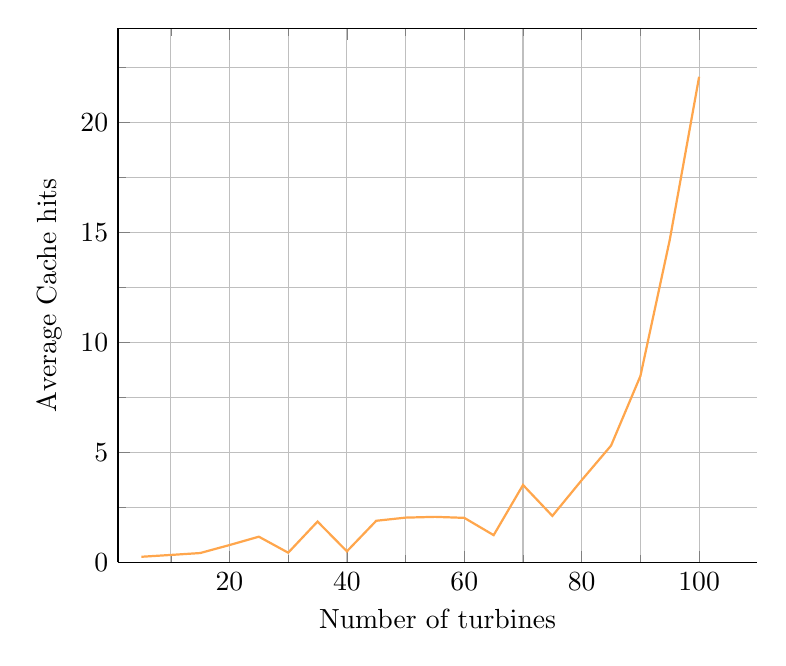
\begin{tikzpicture}
\begin{axis}
[
width=\resultsFigureWidthScale\textwidth,
axis y line*=left,
xlabel=Number of turbines,
ymin = 0,
xmin = 1,
ylabel=Average Cache hits,
%xtick={1, 2, 3, 4, 5, 6, 7, 8, 9, 10, 11, 12, 13, 14, 15, 16, 17, 18, 19, 20},
%xticklabels={5, 10, 15, 20, 25, 30, 35, 40, 45, 50, 55, 60, 65, 70, 75, 80, 85, 90, 95, 100},
%boxplot/draw direction=y,
grid=both,
minor tick num=1
]
%\buildBoxPlot[black]{0}{0}{0}{0}{0}
%\buildBoxPlot[black]{0}{0}{0}{0}{0}
%\buildBoxPlot[black]{0}{0}{0}{0}{0}
%\buildBoxPlot[black]{0}{0}{0}{0}{0}
%\buildBoxPlot[black]{0}{0}{0}{0}{0}
%\buildBoxPlot[black]{0}{0}{0}{0}{0}
%\buildBoxPlot[black]{0}{0}{0}{0}{0}
%\buildBoxPlot[black]{0}{0}{0}{0}{0}
%\buildBoxPlot[black]{0}{0}{0}{0}{0}
%\buildBoxPlot[black]{0}{0}{0}{0}{0}
%\buildBoxPlot[black]{0}{0}{0}{0}{0}
%\buildBoxPlot[black]{0}{0}{0}{0}{0}
%\buildBoxPlot[black]{0}{0}{0}{0}{0}
%\buildBoxPlot[black]{0}{0}{0}{0}{0}
%\buildBoxPlot[black]{0}{0}{0}{0}{0}
%\buildBoxPlot[black]{0}{0}{0}{0}{0}
%\buildBoxPlot[black]{0}{0}{0}{0}{0}
%\buildBoxPlot[black]{0}{0}{0}{0}{0}
%\buildBoxPlot[black]{0}{0}{0}{0}{0}
%\buildBoxPlot[black]{0}{0}{0}{0}{0}
\addplot[thick, orange!70] coordinates {
	(5 ,0.2591015249347438)
	(10 ,0.3423283799799435)
	(15 ,0.4286200856364344)
	(20 ,0.7913519050319182)
	(25 ,1.171919068056407)
	(30 ,0.4440826120490188)
	(35 ,1.8595523144717856)
	(40 ,0.506366007056297)
	(45 ,1.8951768000539848)
	(50 ,2.037951753081981)
	(55 ,2.0728170589196186)
	(60 ,2.0275369832294468)
	(65 ,1.2416290071090674)
	(70 ,3.5220372523313626)
	(75 ,2.115832267020478)
	(80 ,3.7417427229878832)
	(85 ,5.311682134712245)
	(90 ,8.473847137142263)
	(95 ,14.663734246038112)
	(100 ,22.06932793366117)
};
\end{axis}
\end{tikzpicture}
	\caption{Decentralized solution variable number of turbines experiment 1}
	\label{fig:exp:decen:turbines_cache}
\end{figure}


\cref{fig:exp:decen:turbines_cache} show the amount of cache reads the simulation had during part 2 of the experiment.
The plot almost lines up with a exponential curve. Also \cref{fig:exp:decen:turbines,fig:exp:decen:turbines_cache} seams to suddenly increase around 65 ms.

\subsection{Discussion}
\label{sec:disc:turbinesVScycletime}
In the current Siemens system the regulation cycle time of a single Park Pilot scales linearly with the number of turbines.
The aim of the decentralized solution is to detach the regulation cycle time from the number of turbines. 
Looking at \cref{fig:exp:decen:turbines} we see that the decentralized solution seems to be independent of the number of turbines, if the number of turbines is sufficiently low.
From 5 to 65 turbines the regulation cycle time is nearly constant at 20 ms.
The near constant regulation cycle time is caused by the fact that the regulation cycle in the decentralized solution is not forced to wait for data before running the regulation algorithm because data is continually shared between turbines. Adding a turbine to the decentralized solution adds an extra turbine state to factor into the setpoint calculation in the regulation algorithm. This and the added network traffic for the new turbine is the consequence of adding new turbines.

When looking at regulation cycle time of the decentralized solution we must also look at the number of cache reads.
As explained in \cref{sec:exp:performance} a cache read happens when a turbine does not provide a new turbine state package before the next regulation cycle is started.
This forces the regulation cycle to use old data read from cache.
Looking at \cref{fig:exp:decen:turbines_cache} we see that the average number of cache reads in the decentralized solution are below 2 and increasing slightly until we reach 65 turbines. From there the number of cache reads increase exponentially.

The increase in regulation cycle time and cache reads when the number of turbines reaches 65 can be explained by the fact that the network equipment of the test setup is approaching maximum throughput capacity which may cause lost or delayed network packages.
Since regulation cycle time in the decentralized system is dependent on the reception time of the oldest turbine state package as explained in \cref{sec:exp:performance} the loss or delay of network packages has a direct impact on regulation cycle time.
Similarly lost or delayed network packages increases the use of cached data. The increased regulation cycle time and cache reads are thus not a limitation of the decentralized solution but a limitation imposed by the test setup. In order to create a realistic comparison we must disregard the results that are a direct effect of the limitations of our test setup.

Disregarding the limitations imposed by the test setup we see that the regulation cycle time is constant. In terms of regulation cycle time the decentralized solution scales indefinitely. As stated above there is a small increase in regulation cycle time for every turbine added because the state of this turbine has to be taken into consideration when calculating new setpoints on all other turbines. This time addition is not visible on \cref{fig:exp:decen:turbines}. Thus the regulation cycle time will be affected by the addition of turbines but the effect is so small that it is indistinguishable by other factors. Looking at the raw test data 

Still disregarding the limitations imposed by the test setup when looking at the scale factor of the number of cache reads we see another result. The number of cache reads increases slowly with a factor of around 1 cache read for every 30 turbines added, which gives a scale factor of $1 / 30 = 0.033$.

The number of cache reads can be reduced by increasing the regulation cycle time as presented in \cref{fig:exp:decen:sleep-cache}.
Thus the factor deciding the time of the regulation cycle is the maximum number of average cache reads accepted for a single regulation cycle.

\section{\ref{PS:Q:Scalability}}

\textit{Will the regulation cycle time of the new decentralized solution scale better than the current Siemens system in terms of number of turbines per Park Pilot?}\newline\newline

\noindent As mentioned in \cref{cha:existingSystem} the centralized solution is a simulation of the current Siemens system. Thus to complete the comparison between the decentralized solution and the current Siemens system, the discussion section of this experiment also contains a discussion with regards to differences between the centralized solution and the current Siemens system (described in \cref{sec:CenAndCurrentSiemensSystemComparison}).

\subsection{Experiment}
\label{subsec:Exper:Scale}

The \ref{PS:Q:Scalability} problem asks for a comparison between the decentralized solution and the current Siemens system, in order to determine which of the systems scales best, in terms of decreasing the coupling between the regulation cycle time and the number of turbines. For this experiment we compare the results of the \ref{PS:Q:Performance} problem with acquired results from the centralized solution. Thus for this comparison, we study how the regulation cycle time changes when increasing the number of turbines for both systems.


\begin{figure}[b]
	%The figure show how regulation time differs central vs decantral
	\centering
	{\sffamily{Centralized approach}}
	\newline
	

{ %The brackets issolate the enviroment

\makeatletter
\ifcsname c@wavenum\endcsname %Only create one counter
\else
	\newcounter{wavenum}
\fi
\makeatother

\newcommand*{\bitvector}[3]{
  \draw[fill=#3] (t_cur) -- ++( .1, .3) -- ++(#2-.2,0) -- ++(.1, -.3)
                         -- ++(-.1,-.3) -- ++(.2-#2,0) -- cycle;
  \path (t_cur) -- node[anchor=mid] {#1} ++(#2,0) node[time] (t_cur) {};
}

% \known{val}{length}
\newcommand*{\known}[2]{
    \bitvector{#1}{#2}{white}
}

% \unknown{length}
\newcommand*{\unknown}[2]{
    \bitvector{#1}{#2}{black!20}
}

% \nextwave{name}
\newcommand{\nextwave}[1]{
  \path (0,\value{wavenum}) node[left] {#1} node[time] (t_cur) {};
  \addtocounter{wavenum}{-1}
}

% \begin{wave}[clkname]{num_waves}{clock_cycles}
\newenvironment{wave}{
  \begin{tikzpicture}[draw=black, yscale=.8,xscale=1]
    \tikzstyle{time}=[coordinate]
    \setlength{\unitlength}{1cm}
    \setcounter{wavenum}{0}
    
}{\end{tikzpicture}}

%%% End of timing.sty

\begin{wave}
 \nextwave{Regulation Time} \unknown{SendData}{2} \known{WaitForData}{5} \unknown{ReciveData}{2} \unknown{Calculate}{2}
\end{wave}
}

	\newline
	
	{\sffamily{Decentralized approach with seperate data reception}}
	

{ %The brackets issolate the enviroment

\makeatletter
\ifcsname c@wavenum\endcsname %Only create one counter
\else
	\newcounter{wavenum}
\fi
\makeatother

\newcommand*{\bitvector}[3]{
  \draw[fill=#3] (t_cur) -- ++( .1, .3) -- ++(#2-.2,0) -- ++(.1, -.3)
                         -- ++(-.1,-.3) -- ++(.2-#2,0) -- cycle;
  \path (t_cur) -- node[anchor=mid](textNode) {#1} ++(#2,0) node[time] (t_cur) {};
}

% \known{val}{length}
\newcommand*{\known}[2]{
    \bitvector{#1}{#2}{white}
}

% \unknown{length}
\newcommand*{\unknown}[2]{
    \bitvector{#1}{#2}{black!20}
}

% \nextwave{name}
\newcommand{\nextwave}[1]{
  %\path (0,\value{wavenum}) node[left] {#1} node[time] (t_cur) {};
  \path (0,\value{wavenum}) node[time] (t_cur) {};
  \addtocounter{wavenum}{-1}
}

%\newcommand{\timeSpanLabel}{
%	\node (CycleTimeLabel) [rectangle, above = 0.25cm of textNode, inner sep=10pt] {CycleTime};	  
%}

\newcommand{\timeSpanLabel}{
	\node (CycleTimeLabel) [rectangle, above = 1.02cm of t_cur, inner sep=0pt] {Regulation cycle time};
}

\newcommand{\timeSpanA}{
	\node (t_timeSpanA) [point, above = 0 of t_cur] {};	  
}

\newcommand{\timeSpanB}{
	\node (t_timeSpanB) [point, above =0 of t_cur] {};
	
	\graph[use existing nodes]{
		t_timeSpanA --[time span=1cm] CycleTimeLabel;
		CycleTimeLabel.south --[time span=-0.24cm] t_timeSpanB;
	}; 
	
}

%%% End of timing.sty

\begin{tikzpicture}[
	point/.style={inner sep=0pt}, %circle,minimum size=2pt,fill=red},
	draw=black, 
	yscale=.8,
	xscale=1,
	hv path/.style={to path={-| (\tikztotarget)}},
	vh path/.style={to path={|- (\tikztotarget)}},
	skip loop v/.style={to path={-- ++(#1,0) |- (\tikztotarget)}},		
	skip loop h/.style={to path={-- ++(0,#1) -| (\tikztotarget)}},
	time span/.style={to path={-- ++(0,#1) -| (\tikztotarget)}},
	graphs/every graph/.style={edges=rounded corners}	
]
	
\tikzstyle{time}=[coordinate]
\setlength{\unitlength}{1cm}
\setcounter{wavenum}{0}

	\nextwave{} \timeSpanA \unknown{readStates}{3} \unknown{calculate}{3} \timeSpanLabel \unknown{setSetpoint}{3} \unknown{sendState}{3} \timeSpanB \known{wait}{2}
	\nextwave{} \known{reciveStates}{14}
\end{tikzpicture}
}

	\caption{Centralized vs decentralized regulation time}
	\label{fig:timingCentralVSDecentral}
\end{figure}

The regulation cycle time of the decentralized solution is defined as the difference between the receive timestamp of the oldest turbine state (tOldestState) received and the timestamp sampled right after, a new turbine state has been sent (tSent):

$$regulation~cycle~time=tSent-tOldestState$$

The timestamp of the oldest turbine state is used to include network traffic in the regulation cycle time. Thus, if the decentralized solution is using cached data this will be reflected in the regulation cycle time, making the comparison between the centralized and decentralized solution more fair. 
%The aim is to compare the regulation cycle time including , therefore the turbine side centralized solution is not measured. This means that the decentralized version is at a slight disadvantage, since .

We use the following box plot type (for \cref{fig:exp:decen:sleep} and \cref{fig:exp:decen:turbines}): The central mark is the median, the edges of the box are the 25th and 75th percentiles, the whiskers extend to the most extreme data points not considered outliers, and outliers are plotted individually. The whisker length is denoted as 1.5 IQR. 

The following procedure is used each time the experiment is performed:

\begin{minipage}{\textwidth}
	\begin{enumerate}
		\item Start the system with N turbines.
		\item Make sure the system is stable.
		\item Start logging regulation cycle time.
		\item Stop logging after \experiemntRunTime.
		\end{enumerate}
\end{minipage}


\subsection{Results}

\begin{figure}[h!]
	\centering
%	\begin{tikzpicture}
\begin{axis}
[
	width=\resultsPlotWidthScale\textwidth,
	axis y line*=left,
	xlabel=Number of turbines,
	ylabel=Regulation cycle time (ms),
	ymin = 0,
	xmin = 1, xmax = 20,
	xtick={1, 2, 3, 4, 5, 6, 7, 8, 9, 10, 11, 12, 13, 14, 15, 16, 17, 18, 19},
	xticklabels={ , , 15, , 25, , 35, , 45, , 55, , 65, , 75, , 85, , 95},
%	xticklabels={5, 10, 15, 20, 25, 30, 35, 40, 45, 50, 55, 60, 65, 70, 75, 80, 85, 90, 95},
	boxplot/draw direction=y,
	ymajorgrids=true,
	yminorgrids=true,
%	minor y tick num=1,
	max space between ticks=17.5
]

%% /home/stefan/work/TestResults/Test4_Centralized_success_12-4-2014_2024/CentralizedLog2.csv
%\buildBoxPlot{0.871522}{0.955}{0.809034}{12.535623}{0.541744}
\buildBoxPlot[black]{0}{0}{0}{0}{0}

%% /home/stefan/work/TestResults/Test4_Centralized_success_12-4-2014_2024/CentralizedLog3.csv
\buildBoxPlot{1.168815}{1.310873}{1.081427}{24.566027}{0.591135}

%% /home/stefan/work/TestResults/Test4_Centralized_success_12-4-2014_2024/CentralizedLog4.csv
\buildBoxPlot{1.398871}{1.613768}{1.303639}{19.188073}{0.747894}

%% /home/stefan/work/TestResults/Test4_Centralized_success_12-4-2014_2024/CentralizedLog5.csv
\buildBoxPlot{1.722236}{1.981776}{1.596331}{13.257023}{1.077214}

%% /home/stefan/work/TestResults/Test4_Centralized_success_12-4-2014_2024/CentralizedLog6.csv
\buildBoxPlot{1.978881}{2.337657}{1.823133}{20.243534}{1.278172}

%% /home/stefan/work/TestResults/Test4_Centralized_success_12-4-2014_2024/CentralizedLog7.csv
\buildBoxPlot{2.985681}{3.527133}{2.724617}{102.89112}{1.917354}

%% /home/stefan/work/TestResults/Test4_Centralized_success_12-4-2014_2024/CentralizedLog8.csv
\buildBoxPlot{5.662268}{6.776311}{5.315074}{55.800126}{3.845115}

%% /home/stefan/work/TestResults/Test4_Centralized_success_12-4-2014_2024/CentralizedLog9.csv
\buildBoxPlot{14.607313}{22.842589}{10.21933}{40.119104}{7.578863}

%% /home/stefan/work/TestResults/Test4_Centralized_success_12-4-2014_2024/CentralizedLog10.csv
\buildBoxPlot{16.673738}{25.382756}{14.810635}{46.844742}{12.042462}

%% /home/stefan/work/TestResults/Test4_Centralized_success_12-4-2014_2024/CentralizedLog11.csv
\buildBoxPlot{20.220936}{27.962488}{19.190067}{63.348974}{17.058657}

%% /home/stefan/work/TestResults/Test4_Centralized_success_12-4-2014_2024/CentralizedLog12.csv
\buildBoxPlot{31.587407}{33.177592}{24.950794}{46.841843}{22.941051}

%% /home/stefan/work/TestResults/Test4_Centralized_success_12-4-2014_2024/CentralizedLog13.csv
\buildBoxPlot{36.93711}{38.790125}{32.230331}{51.398495}{29.702809}

%% /home/stefan/work/TestResults/Test4_Centralized_success_12-4-2014_2024/CentralizedLog14.csv
\buildBoxPlot{40.231022}{42.885333}{36.673407}{77.051599}{33.854906}

%% /home/stefan/work/TestResults/Test4_Centralized_success_12-4-2014_2024/CentralizedLog15.csv
\buildBoxPlot{45.380062}{48.694656}{42.841453}{225.894089}{39.402015}

%% /home/stefan/work/TestResults/Test4_Centralized_success_12-4-2014_2024/CentralizedLog16.csv
\buildBoxPlot{51.425649}{54.462315}{48.438981}{250.200229}{45.062697}

%% /home/stefan/work/TestResults/Test4_Centralized_success_12-4-2014_2024/CentralizedLog17.csv
\buildBoxPlot{58.196177}{62.557505}{55.582236}{271.626595}{51.598593}

%% /home/stefan/work/TestResults/Test4_Centralized_success_12-4-2014_2024/CentralizedLog18.csv
\buildBoxPlot{64.70376}{70.553035}{62.053219}{278.866888}{57.401402}

%% /home/stefan/work/TestResults/Test4_Centralized_success_12-4-2014_2024/CentralizedLog19.csv
\buildBoxPlot{73.715686}{80.566923}{69.809765}{287.542878}{65.698499}

%% /home/stefan/work/TestResults/Test4_Centralized_success_12-4-2014_2024/CentralizedLog20.csv
\buildBoxPlot{82.961949}{151.608592}{77.825807}{290.243704}{72.589561}


\addplot[thick, red!70] coordinates {
%	(1 ,0.871522)
	(2 ,1.168815)
	(3 ,1.398871)
	(4 ,1.722236)
	(5 ,1.978881)
	(6 ,2.985681)
	(7 ,5.662268)
	(8 ,14.607313)
	(9 ,16.673738)
	(10 ,20.220936)
	(11 ,31.587407)
	(12 ,36.93711)
	(13 ,40.231022)
	(14 ,45.380062)
	(15 ,51.425649)
	(16 ,58.196177)
	(17 ,64.70376)
	(18 ,73.715686)
	(19 ,82.961949)
};

\end{axis}
\end{tikzpicture}

%	% This file was created by matlab2tikz.
% Minimal pgfplots version: 1.3
%
%The latest updates can be retrieved from
%  http://www.mathworks.com/matlabcentral/fileexchange/22022-matlab2tikz
%where you can also make suggestions and rate matlab2tikz.
%
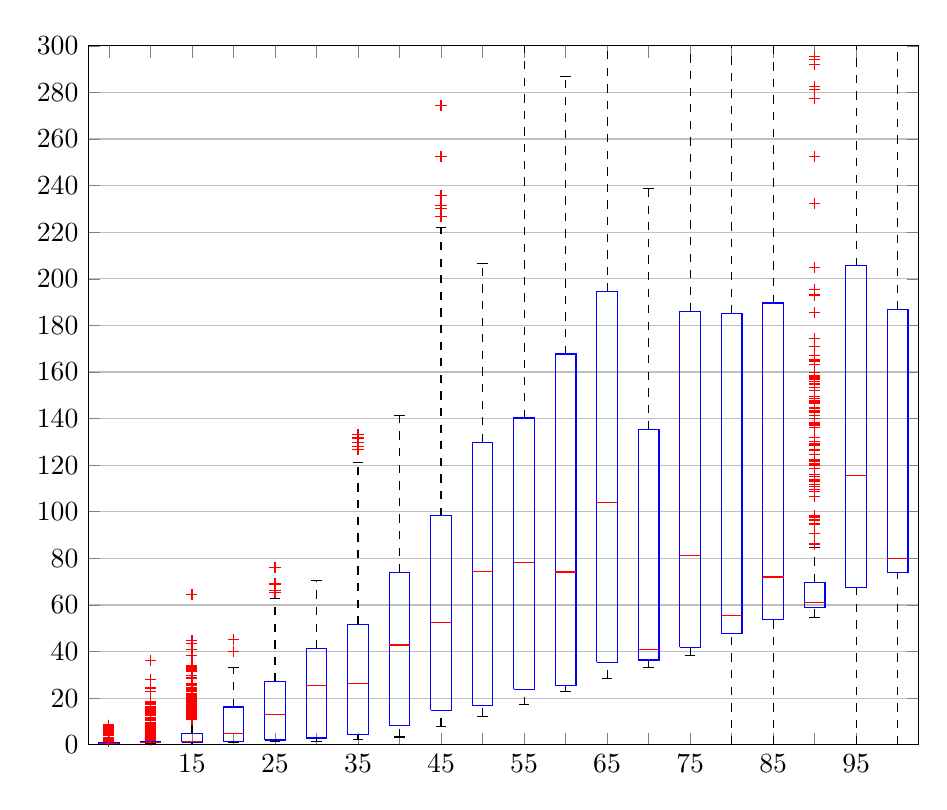
\begin{tikzpicture}

\begin{axis}[%
	width=\resultsPlotWidthScale\textwidth,
	xmin=0.5,
	xmax=20.5,
	xtick={1, 2, 3, 4, 5, 6, 7, 8, 9, 10, 11, 12, 13, 14, 15, 16, 17, 18, 19},
	xticklabels={ , , 15, , 25, , 35, , 45, , 55, , 65, , 75, , 85, , 95},
	ymin=0,
	ymax=300,
	ymajorgrids=true,
	yminorgrids=true,
	max space between ticks=17.5
]
\addplot [color=black,dashed,forget plot]
  table[row sep=crcr]{%
1	0.8717095\\
1	1.204627\\
};
\addplot [color=black,dashed,forget plot]
  table[row sep=crcr]{%
2	1.2604475\\
2	1.888937\\
};
\addplot [color=black,dashed,forget plot]
  table[row sep=crcr]{%
3	4.944662\\
3	10.675016\\
};
\addplot [color=black,dashed,forget plot]
  table[row sep=crcr]{%
4	16.2032205\\
4	33.311733\\
};
\addplot [color=black,dashed,forget plot]
  table[row sep=crcr]{%
5	27.053618\\
5	62.899558\\
};
\addplot [color=black,dashed,forget plot]
  table[row sep=crcr]{%
6	41.2910465\\
6	70.350287\\
};
\addplot [color=black,dashed,forget plot]
  table[row sep=crcr]{%
7	51.581584\\
7	121.085436\\
};
\addplot [color=black,dashed,forget plot]
  table[row sep=crcr]{%
8	73.910551\\
8	141.135822\\
};
\addplot [color=black,dashed,forget plot]
  table[row sep=crcr]{%
9	98.232932\\
9	222.18631\\
};
\addplot [color=black,dashed,forget plot]
  table[row sep=crcr]{%
10	129.9151\\
10	206.701738\\
};
\addplot [color=black,dashed,forget plot]
  table[row sep=crcr]{%
11	140.2385985\\
11	307.003647\\
};
\addplot [color=black,dashed,forget plot]
  table[row sep=crcr]{%
12	167.7148685\\
12	286.824347\\
};
\addplot [color=black,dashed,forget plot]
  table[row sep=crcr]{%
13	194.42233\\
13	426.984091\\
};
\addplot [color=black,dashed,forget plot]
  table[row sep=crcr]{%
14	135.221256\\
14	238.898358\\
};
\addplot [color=black,dashed,forget plot]
  table[row sep=crcr]{%
15	185.872368\\
15	399.208961\\
};
\addplot [color=black,dashed,forget plot]
  table[row sep=crcr]{%
16	185.049093\\
16	387.933056\\
};
\addplot [color=black,dashed,forget plot]
  table[row sep=crcr]{%
17	189.620724\\
17	390.403391\\
};
\addplot [color=black,dashed,forget plot]
  table[row sep=crcr]{%
18	69.756227\\
18	84.575222\\
};
\addplot [color=black,dashed,forget plot]
  table[row sep=crcr]{%
19	205.557893\\
19	412.155966\\
};
\addplot [color=black,dashed,forget plot]
  table[row sep=crcr]{%
20	186.7835205\\
20	355.119078\\
};
\addplot [color=black,dashed,forget plot]
  table[row sep=crcr]{%
1	0.452249\\
1	0.6489595\\
};
\addplot [color=black,dashed,forget plot]
  table[row sep=crcr]{%
2	0.604707\\
2	0.8393005\\
};
\addplot [color=black,dashed,forget plot]
  table[row sep=crcr]{%
3	0\\
3	1.1243275\\
};
\addplot [color=black,dashed,forget plot]
  table[row sep=crcr]{%
4	1.021879\\
4	1.5244415\\
};
\addplot [color=black,dashed,forget plot]
  table[row sep=crcr]{%
5	1.244611\\
5	2.061173\\
};
\addplot [color=black,dashed,forget plot]
  table[row sep=crcr]{%
6	1.524188\\
6	2.90871\\
};
\addplot [color=black,dashed,forget plot]
  table[row sep=crcr]{%
7	2.156496\\
7	4.2507545\\
};
\addplot [color=black,dashed,forget plot]
  table[row sep=crcr]{%
8	3.330849\\
8	8.282937\\
};
\addplot [color=black,dashed,forget plot]
  table[row sep=crcr]{%
9	7.831812\\
9	14.81487\\
};
\addplot [color=black,dashed,forget plot]
  table[row sep=crcr]{%
10	12.246399\\
10	16.6843555\\
};
\addplot [color=black,dashed,forget plot]
  table[row sep=crcr]{%
11	17.135656\\
11	23.771084\\
};
\addplot [color=black,dashed,forget plot]
  table[row sep=crcr]{%
12	22.778828\\
12	25.513819\\
};
\addplot [color=black,dashed,forget plot]
  table[row sep=crcr]{%
13	28.467515\\
13	35.4142585\\
};
\addplot [color=black,dashed,forget plot]
  table[row sep=crcr]{%
14	33.316406\\
14	36.380356\\
};
\addplot [color=black,dashed,forget plot]
  table[row sep=crcr]{%
15	38.153571\\
15	41.905524\\
};
\addplot [color=black,dashed,forget plot]
  table[row sep=crcr]{%
16	0\\
16	47.5835365\\
};
\addplot [color=black,dashed,forget plot]
  table[row sep=crcr]{%
17	0\\
17	53.6428275\\
};
\addplot [color=black,dashed,forget plot]
  table[row sep=crcr]{%
18	54.565993\\
18	58.849282\\
};
\addplot [color=black,dashed,forget plot]
  table[row sep=crcr]{%
19	0\\
19	67.47031\\
};
\addplot [color=black,dashed,forget plot]
  table[row sep=crcr]{%
20	0\\
20	74.0472365\\
};
\addplot [color=black,solid,forget plot]
  table[row sep=crcr]{%
0.875	1.204627\\
1.125	1.204627\\
};
\addplot [color=black,solid,forget plot]
  table[row sep=crcr]{%
1.875	1.888937\\
2.125	1.888937\\
};
\addplot [color=black,solid,forget plot]
  table[row sep=crcr]{%
2.875	10.675016\\
3.125	10.675016\\
};
\addplot [color=black,solid,forget plot]
  table[row sep=crcr]{%
3.875	33.311733\\
4.125	33.311733\\
};
\addplot [color=black,solid,forget plot]
  table[row sep=crcr]{%
4.875	62.899558\\
5.125	62.899558\\
};
\addplot [color=black,solid,forget plot]
  table[row sep=crcr]{%
5.875	70.350287\\
6.125	70.350287\\
};
\addplot [color=black,solid,forget plot]
  table[row sep=crcr]{%
6.875	121.085436\\
7.125	121.085436\\
};
\addplot [color=black,solid,forget plot]
  table[row sep=crcr]{%
7.875	141.135822\\
8.125	141.135822\\
};
\addplot [color=black,solid,forget plot]
  table[row sep=crcr]{%
8.875	222.18631\\
9.125	222.18631\\
};
\addplot [color=black,solid,forget plot]
  table[row sep=crcr]{%
9.875	206.701738\\
10.125	206.701738\\
};
\addplot [color=black,solid,forget plot]
  table[row sep=crcr]{%
10.875	307.003647\\
11.125	307.003647\\
};
\addplot [color=black,solid,forget plot]
  table[row sep=crcr]{%
11.875	286.824347\\
12.125	286.824347\\
};
\addplot [color=black,solid,forget plot]
  table[row sep=crcr]{%
12.875	426.984091\\
13.125	426.984091\\
};
\addplot [color=black,solid,forget plot]
  table[row sep=crcr]{%
13.875	238.898358\\
14.125	238.898358\\
};
\addplot [color=black,solid,forget plot]
  table[row sep=crcr]{%
14.875	399.208961\\
15.125	399.208961\\
};
\addplot [color=black,solid,forget plot]
  table[row sep=crcr]{%
15.875	387.933056\\
16.125	387.933056\\
};
\addplot [color=black,solid,forget plot]
  table[row sep=crcr]{%
16.875	390.403391\\
17.125	390.403391\\
};
\addplot [color=black,solid,forget plot]
  table[row sep=crcr]{%
17.875	84.575222\\
18.125	84.575222\\
};
\addplot [color=black,solid,forget plot]
  table[row sep=crcr]{%
18.875	412.155966\\
19.125	412.155966\\
};
\addplot [color=black,solid,forget plot]
  table[row sep=crcr]{%
19.875	355.119078\\
20.125	355.119078\\
};
\addplot [color=black,solid,forget plot]
  table[row sep=crcr]{%
0.875	0.452249\\
1.125	0.452249\\
};
\addplot [color=black,solid,forget plot]
  table[row sep=crcr]{%
1.875	0.604707\\
2.125	0.604707\\
};
\addplot [color=black,solid,forget plot]
  table[row sep=crcr]{%
2.875	0\\
3.125	0\\
};
\addplot [color=black,solid,forget plot]
  table[row sep=crcr]{%
3.875	1.021879\\
4.125	1.021879\\
};
\addplot [color=black,solid,forget plot]
  table[row sep=crcr]{%
4.875	1.244611\\
5.125	1.244611\\
};
\addplot [color=black,solid,forget plot]
  table[row sep=crcr]{%
5.875	1.524188\\
6.125	1.524188\\
};
\addplot [color=black,solid,forget plot]
  table[row sep=crcr]{%
6.875	2.156496\\
7.125	2.156496\\
};
\addplot [color=black,solid,forget plot]
  table[row sep=crcr]{%
7.875	3.330849\\
8.125	3.330849\\
};
\addplot [color=black,solid,forget plot]
  table[row sep=crcr]{%
8.875	7.831812\\
9.125	7.831812\\
};
\addplot [color=black,solid,forget plot]
  table[row sep=crcr]{%
9.875	12.246399\\
10.125	12.246399\\
};
\addplot [color=black,solid,forget plot]
  table[row sep=crcr]{%
10.875	17.135656\\
11.125	17.135656\\
};
\addplot [color=black,solid,forget plot]
  table[row sep=crcr]{%
11.875	22.778828\\
12.125	22.778828\\
};
\addplot [color=black,solid,forget plot]
  table[row sep=crcr]{%
12.875	28.467515\\
13.125	28.467515\\
};
\addplot [color=black,solid,forget plot]
  table[row sep=crcr]{%
13.875	33.316406\\
14.125	33.316406\\
};
\addplot [color=black,solid,forget plot]
  table[row sep=crcr]{%
14.875	38.153571\\
15.125	38.153571\\
};
\addplot [color=black,solid,forget plot]
  table[row sep=crcr]{%
15.875	0\\
16.125	0\\
};
\addplot [color=black,solid,forget plot]
  table[row sep=crcr]{%
16.875	0\\
17.125	0\\
};
\addplot [color=black,solid,forget plot]
  table[row sep=crcr]{%
17.875	54.565993\\
18.125	54.565993\\
};
\addplot [color=black,solid,forget plot]
  table[row sep=crcr]{%
18.875	0\\
19.125	0\\
};
\addplot [color=black,solid,forget plot]
  table[row sep=crcr]{%
19.875	0\\
20.125	0\\
};
\addplot [color=blue,solid,forget plot]
  table[row sep=crcr]{%
0.75	0.6489595\\
0.75	0.8717095\\
1.25	0.8717095\\
1.25	0.6489595\\
0.75	0.6489595\\
};
\addplot [color=blue,solid,forget plot]
  table[row sep=crcr]{%
1.75	0.8393005\\
1.75	1.2604475\\
2.25	1.2604475\\
2.25	0.8393005\\
1.75	0.8393005\\
};
\addplot [color=blue,solid,forget plot]
  table[row sep=crcr]{%
2.75	1.1243275\\
2.75	4.944662\\
3.25	4.944662\\
3.25	1.1243275\\
2.75	1.1243275\\
};
\addplot [color=blue,solid,forget plot]
  table[row sep=crcr]{%
3.75	1.5244415\\
3.75	16.2032205\\
4.25	16.2032205\\
4.25	1.5244415\\
3.75	1.5244415\\
};
\addplot [color=blue,solid,forget plot]
  table[row sep=crcr]{%
4.75	2.061173\\
4.75	27.053618\\
5.25	27.053618\\
5.25	2.061173\\
4.75	2.061173\\
};
\addplot [color=blue,solid,forget plot]
  table[row sep=crcr]{%
5.75	2.90871\\
5.75	41.2910465\\
6.25	41.2910465\\
6.25	2.90871\\
5.75	2.90871\\
};
\addplot [color=blue,solid,forget plot]
  table[row sep=crcr]{%
6.75	4.2507545\\
6.75	51.581584\\
7.25	51.581584\\
7.25	4.2507545\\
6.75	4.2507545\\
};
\addplot [color=blue,solid,forget plot]
  table[row sep=crcr]{%
7.75	8.282937\\
7.75	73.910551\\
8.25	73.910551\\
8.25	8.282937\\
7.75	8.282937\\
};
\addplot [color=blue,solid,forget plot]
  table[row sep=crcr]{%
8.75	14.81487\\
8.75	98.232932\\
9.25	98.232932\\
9.25	14.81487\\
8.75	14.81487\\
};
\addplot [color=blue,solid,forget plot]
  table[row sep=crcr]{%
9.75	16.6843555\\
9.75	129.9151\\
10.25	129.9151\\
10.25	16.6843555\\
9.75	16.6843555\\
};
\addplot [color=blue,solid,forget plot]
  table[row sep=crcr]{%
10.75	23.771084\\
10.75	140.2385985\\
11.25	140.2385985\\
11.25	23.771084\\
10.75	23.771084\\
};
\addplot [color=blue,solid,forget plot]
  table[row sep=crcr]{%
11.75	25.513819\\
11.75	167.7148685\\
12.25	167.7148685\\
12.25	25.513819\\
11.75	25.513819\\
};
\addplot [color=blue,solid,forget plot]
  table[row sep=crcr]{%
12.75	35.4142585\\
12.75	194.42233\\
13.25	194.42233\\
13.25	35.4142585\\
12.75	35.4142585\\
};
\addplot [color=blue,solid,forget plot]
  table[row sep=crcr]{%
13.75	36.380356\\
13.75	135.221256\\
14.25	135.221256\\
14.25	36.380356\\
13.75	36.380356\\
};
\addplot [color=blue,solid,forget plot]
  table[row sep=crcr]{%
14.75	41.905524\\
14.75	185.872368\\
15.25	185.872368\\
15.25	41.905524\\
14.75	41.905524\\
};
\addplot [color=blue,solid,forget plot]
  table[row sep=crcr]{%
15.75	47.5835365\\
15.75	185.049093\\
16.25	185.049093\\
16.25	47.5835365\\
15.75	47.5835365\\
};
\addplot [color=blue,solid,forget plot]
  table[row sep=crcr]{%
16.75	53.6428275\\
16.75	189.620724\\
17.25	189.620724\\
17.25	53.6428275\\
16.75	53.6428275\\
};
\addplot [color=blue,solid,forget plot]
  table[row sep=crcr]{%
17.75	58.849282\\
17.75	69.756227\\
18.25	69.756227\\
18.25	58.849282\\
17.75	58.849282\\
};
\addplot [color=blue,solid,forget plot]
  table[row sep=crcr]{%
18.75	67.47031\\
18.75	205.557893\\
19.25	205.557893\\
19.25	67.47031\\
18.75	67.47031\\
};
\addplot [color=blue,solid,forget plot]
  table[row sep=crcr]{%
19.75	74.0472365\\
19.75	186.7835205\\
20.25	186.7835205\\
20.25	74.0472365\\
19.75	74.0472365\\
};
\addplot [color=red,solid,forget plot]
  table[row sep=crcr]{%
0.75	0.727033\\
1.25	0.727033\\
};
\addplot [color=red,solid,forget plot]
  table[row sep=crcr]{%
1.75	0.9325085\\
2.25	0.9325085\\
};
\addplot [color=red,solid,forget plot]
  table[row sep=crcr]{%
2.75	1.3743515\\
3.25	1.3743515\\
};
\addplot [color=red,solid,forget plot]
  table[row sep=crcr]{%
3.75	4.791979\\
4.25	4.791979\\
};
\addplot [color=red,solid,forget plot]
  table[row sep=crcr]{%
4.75	13.090375\\
5.25	13.090375\\
};
\addplot [color=red,solid,forget plot]
  table[row sep=crcr]{%
5.75	25.5858225\\
6.25	25.5858225\\
};
\addplot [color=red,solid,forget plot]
  table[row sep=crcr]{%
6.75	26.3139895\\
7.25	26.3139895\\
};
\addplot [color=red,solid,forget plot]
  table[row sep=crcr]{%
7.75	42.7994295\\
8.25	42.7994295\\
};
\addplot [color=red,solid,forget plot]
  table[row sep=crcr]{%
8.75	52.370321\\
9.25	52.370321\\
};
\addplot [color=red,solid,forget plot]
  table[row sep=crcr]{%
9.75	74.509338\\
10.25	74.509338\\
};
\addplot [color=red,solid,forget plot]
  table[row sep=crcr]{%
10.75	78.4097345\\
11.25	78.4097345\\
};
\addplot [color=red,solid,forget plot]
  table[row sep=crcr]{%
11.75	74.1398775\\
12.25	74.1398775\\
};
\addplot [color=red,solid,forget plot]
  table[row sep=crcr]{%
12.75	103.919405\\
13.25	103.919405\\
};
\addplot [color=red,solid,forget plot]
  table[row sep=crcr]{%
13.75	40.8226565\\
14.25	40.8226565\\
};
\addplot [color=red,solid,forget plot]
  table[row sep=crcr]{%
14.75	81.151909\\
15.25	81.151909\\
};
\addplot [color=red,solid,forget plot]
  table[row sep=crcr]{%
15.75	55.4174655\\
16.25	55.4174655\\
};
\addplot [color=red,solid,forget plot]
  table[row sep=crcr]{%
16.75	71.9904755\\
17.25	71.9904755\\
};
\addplot [color=red,solid,forget plot]
  table[row sep=crcr]{%
17.75	60.9902745\\
18.25	60.9902745\\
};
\addplot [color=red,solid,forget plot]
  table[row sep=crcr]{%
18.75	115.484537\\
19.25	115.484537\\
};
\addplot [color=red,solid,forget plot]
  table[row sep=crcr]{%
19.75	79.967163\\
20.25	79.967163\\
};
\addplot [color=blue,only marks,mark=+,mark options={solid,draw=red},forget plot]
  table[row sep=crcr]{%
1	1.22142\\
1	1.223364\\
1	1.224134\\
1	1.233426\\
1	1.238923\\
1	1.249099\\
1	1.267809\\
1	1.284091\\
1	1.291981\\
1	1.319801\\
1	1.336661\\
1	1.415403\\
1	1.421902\\
1	1.503776\\
1	1.51294\\
1	1.532207\\
1	1.546875\\
1	1.547268\\
1	1.584143\\
1	1.589388\\
1	1.638589\\
1	1.811361\\
1	1.830223\\
1	1.831018\\
1	1.831122\\
1	1.835368\\
1	1.844371\\
1	2.105473\\
1	2.236183\\
1	2.251674\\
1	2.280143\\
1	2.299661\\
1	2.522178\\
1	2.750071\\
1	2.792578\\
1	3.25494\\
1	3.2941\\
1	3.929381\\
1	3.990809\\
1	4.137583\\
1	4.472371\\
1	4.537438\\
1	5.003565\\
1	5.006466\\
1	5.080215\\
1	5.089503\\
1	5.200881\\
1	5.250616\\
1	5.546884\\
1	5.625184\\
1	5.774674\\
1	5.797138\\
1	5.85168\\
1	5.899315\\
1	6.016238\\
1	6.033693\\
1	6.065686\\
1	6.074834\\
1	6.090889\\
1	6.127169\\
1	6.155085\\
1	6.426519\\
1	6.448381\\
1	6.519414\\
1	6.550741\\
1	6.582032\\
1	6.600282\\
1	6.737918\\
1	6.745443\\
1	6.750611\\
1	6.789309\\
1	6.798253\\
1	6.822493\\
1	6.995045\\
1	7.029346\\
1	7.053232\\
1	7.064158\\
1	7.07522\\
1	7.135983\\
1	7.160974\\
1	7.188216\\
1	7.222805\\
1	7.233565\\
1	7.249176\\
1	7.249689\\
1	7.27116\\
1	7.325184\\
1	7.352011\\
1	7.389161\\
1	7.426482\\
1	7.431757\\
1	7.463729\\
1	7.47152\\
1	7.522566\\
1	7.535727\\
1	7.545131\\
1	7.574998\\
1	7.635756\\
1	7.637039\\
1	7.681288\\
1	7.69941\\
1	7.713476\\
1	7.746304\\
1	7.80394\\
1	7.820249\\
1	7.866035\\
1	7.880942\\
1	7.974198\\
1	7.996921\\
1	8.016012\\
1	8.038029\\
1	8.038785\\
1	8.043832\\
1	8.054257\\
1	8.068841\\
1	8.094754\\
1	8.09828\\
1	8.100322\\
1	8.14914\\
1	8.165973\\
1	8.168417\\
1	8.197402\\
1	8.204572\\
1	8.211569\\
1	8.273737\\
1	8.292364\\
1	8.31482\\
1	8.323623\\
1	8.324661\\
1	8.35753\\
1	8.36441\\
1	8.443329\\
1	8.458258\\
};
\addplot [color=blue,only marks,mark=+,mark options={solid,draw=red},forget plot]
  table[row sep=crcr]{%
2	1.90167\\
2	1.911317\\
2	1.962956\\
2	1.968191\\
2	1.985629\\
2	1.990298\\
2	1.99821\\
2	1.999762\\
2	2.006972\\
2	2.01125\\
2	2.016703\\
2	2.060781\\
2	2.078726\\
2	2.084904\\
2	2.0886\\
2	2.149672\\
2	2.152386\\
2	2.157416\\
2	2.172206\\
2	2.210438\\
2	2.211897\\
2	2.265665\\
2	2.319203\\
2	2.320914\\
2	2.349612\\
2	2.398934\\
2	2.415953\\
2	2.462345\\
2	2.517542\\
2	2.518407\\
2	2.522352\\
2	2.559802\\
2	2.55986\\
2	2.588216\\
2	2.616982\\
2	2.640217\\
2	2.728957\\
2	2.763691\\
2	2.781829\\
2	2.796268\\
2	2.805757\\
2	2.809971\\
2	2.835864\\
2	2.857655\\
2	2.898538\\
2	2.902265\\
2	2.93052\\
2	2.958764\\
2	2.970508\\
2	2.981127\\
2	2.987679\\
2	2.993292\\
2	2.996044\\
2	3.003311\\
2	3.040946\\
2	3.044832\\
2	3.159759\\
2	3.171292\\
2	3.19803\\
2	3.223353\\
2	3.282729\\
2	3.322616\\
2	3.368547\\
2	3.522944\\
2	3.548358\\
2	3.57788\\
2	3.588871\\
2	3.709183\\
2	3.753555\\
2	4.156216\\
2	4.158493\\
2	4.17583\\
2	4.215829\\
2	4.22159\\
2	4.303591\\
2	4.378721\\
2	4.432432\\
2	4.496267\\
2	4.535655\\
2	4.562851\\
2	4.603645\\
2	4.626893\\
2	4.675847\\
2	4.697096\\
2	4.700302\\
2	4.704188\\
2	4.712042\\
2	4.793507\\
2	4.815152\\
2	4.857104\\
2	4.903281\\
2	4.925399\\
2	4.947763\\
2	5.141249\\
2	5.193353\\
2	5.338926\\
2	5.457376\\
2	5.767504\\
2	5.946886\\
2	6.065162\\
2	6.27828\\
2	6.380513\\
2	6.388238\\
2	6.414966\\
2	6.488282\\
2	6.659254\\
2	6.683566\\
2	6.877373\\
2	6.964909\\
2	7.118723\\
2	7.150523\\
2	7.184356\\
2	7.355692\\
2	7.373073\\
2	7.375065\\
2	7.387138\\
2	7.610728\\
2	7.827468\\
2	7.997416\\
2	8.003218\\
2	8.194986\\
2	8.875918\\
2	9.030813\\
2	9.168052\\
2	9.234478\\
2	9.240843\\
2	9.32023\\
2	9.355343\\
2	9.585629\\
2	9.632804\\
2	10.256122\\
2	10.54318\\
2	10.803498\\
2	10.849408\\
2	10.856044\\
2	10.946935\\
2	11.105923\\
2	11.112722\\
2	11.34085\\
2	11.612397\\
2	11.670481\\
2	11.712875\\
2	12.553934\\
2	12.558786\\
2	12.600901\\
2	12.730505\\
2	13.03436\\
2	13.59391\\
2	13.644562\\
2	14.067884\\
2	14.353523\\
2	14.417325\\
2	14.694076\\
2	14.763316\\
2	14.969792\\
2	14.992874\\
2	15.324704\\
2	15.355964\\
2	15.496052\\
2	15.989522\\
2	16.258874\\
2	16.543165\\
2	17.449576\\
2	17.943462\\
2	18.002392\\
2	18.307749\\
2	18.434977\\
2	22.673764\\
2	22.875711\\
2	24.368586\\
2	28.112777\\
2	36.326413\\
};
\addplot [color=blue,only marks,mark=+,mark options={solid,draw=red},forget plot]
  table[row sep=crcr]{%
3	10.712372\\
3	10.72463\\
3	10.824215\\
3	10.912497\\
3	10.934032\\
3	10.970966\\
3	11.133457\\
3	11.216931\\
3	11.239228\\
3	11.326209\\
3	11.337168\\
3	11.358172\\
3	11.440343\\
3	11.469403\\
3	11.51297\\
3	11.534249\\
3	11.610081\\
3	11.663412\\
3	11.694482\\
3	11.764268\\
3	11.788597\\
3	11.879232\\
3	11.88636\\
3	11.895998\\
3	11.951678\\
3	11.962575\\
3	12.136279\\
3	12.172993\\
3	12.18119\\
3	12.246693\\
3	12.301922\\
3	12.397148\\
3	12.649651\\
3	12.679065\\
3	12.736198\\
3	12.783409\\
3	12.846494\\
3	12.904049\\
3	12.983231\\
3	12.990299\\
3	12.999456\\
3	13.019261\\
3	13.133643\\
3	13.214978\\
3	13.294728\\
3	13.312276\\
3	13.361947\\
3	13.63175\\
3	13.636207\\
3	13.644932\\
3	13.834311\\
3	13.89846\\
3	13.935251\\
3	13.936967\\
3	13.984923\\
3	14.005203\\
3	14.066154\\
3	14.181378\\
3	14.216491\\
3	14.269401\\
3	14.371669\\
3	14.381037\\
3	14.391874\\
3	14.394386\\
3	14.406414\\
3	14.524739\\
3	14.653434\\
3	14.755178\\
3	14.874585\\
3	14.876075\\
3	15.017429\\
3	15.156781\\
3	15.305643\\
3	15.349046\\
3	15.516102\\
3	15.536637\\
3	15.593484\\
3	15.722859\\
3	16.133056\\
3	16.151682\\
3	16.251942\\
3	16.652387\\
3	16.82844\\
3	16.830175\\
3	16.845397\\
3	16.963685\\
3	17.027354\\
3	17.126082\\
3	17.175433\\
3	17.441423\\
3	17.447871\\
3	17.503013\\
3	18.054716\\
3	18.218939\\
3	18.232524\\
3	18.412774\\
3	18.471894\\
3	18.535344\\
3	18.547782\\
3	19.067263\\
3	19.288464\\
3	19.337552\\
3	19.550863\\
3	19.553737\\
3	19.65005\\
3	19.89144\\
3	20.004595\\
3	20.030844\\
3	20.076484\\
3	20.148205\\
3	20.24326\\
3	20.369406\\
3	20.548091\\
3	20.577104\\
3	20.989983\\
3	21.035488\\
3	21.265652\\
3	21.308726\\
3	21.391766\\
3	21.467402\\
3	21.487734\\
3	21.706475\\
3	21.806243\\
3	21.837835\\
3	21.847035\\
3	22.749871\\
3	23.003556\\
3	23.117597\\
3	23.162438\\
3	23.195855\\
3	23.466837\\
3	23.49557\\
3	23.627204\\
3	24.374648\\
3	24.422942\\
3	25.351046\\
3	25.782507\\
3	25.823924\\
3	25.873848\\
3	26.10141\\
3	26.481113\\
3	28.651801\\
3	28.687621\\
3	28.930998\\
3	29.6302\\
3	29.797236\\
3	31.334925\\
3	31.747665\\
3	32.48028\\
3	32.619401\\
3	33.017111\\
3	33.299365\\
3	33.710997\\
3	34.202288\\
3	38.391179\\
3	41.073174\\
3	43.384782\\
3	44.587852\\
3	44.822243\\
3	64.609355\\
};
\addplot [color=blue,only marks,mark=+,mark options={solid,draw=red},forget plot]
  table[row sep=crcr]{%
4	39.999706\\
4	45.044395\\
};
\addplot [color=blue,only marks,mark=+,mark options={solid,draw=red},forget plot]
  table[row sep=crcr]{%
5	65.437522\\
5	66.282007\\
5	68.917478\\
5	69.027589\\
5	69.32905\\
5	76.022717\\
};
\addplot [color=blue,only marks,mark=+,mark options={solid,draw=red},forget plot]
  table[row sep=crcr]{%
nan	nan\\
};
\addplot [color=blue,only marks,mark=+,mark options={solid,draw=red},forget plot]
  table[row sep=crcr]{%
7	126.57364\\
7	127.839887\\
7	129.633535\\
7	131.39321\\
7	131.744755\\
7	132.993896\\
};
\addplot [color=blue,only marks,mark=+,mark options={solid,draw=red},forget plot]
  table[row sep=crcr]{%
nan	nan\\
};
\addplot [color=blue,only marks,mark=+,mark options={solid,draw=red},forget plot]
  table[row sep=crcr]{%
9	226.846077\\
9	230.029879\\
9	231.330554\\
9	235.828114\\
9	252.531861\\
9	274.415257\\
};
\addplot [color=blue,only marks,mark=+,mark options={solid,draw=red},forget plot]
  table[row sep=crcr]{%
nan	nan\\
};
\addplot [color=blue,only marks,mark=+,mark options={solid,draw=red},forget plot]
  table[row sep=crcr]{%
11	328.644114\\
11	334.633811\\
11	347.48941\\
11	352.28358\\
};
\addplot [color=blue,only marks,mark=+,mark options={solid,draw=red},forget plot]
  table[row sep=crcr]{%
12	466.979415\\
12	790.974015\\
12	799.073064\\
12	807.138983\\
12	811.776466\\
12	825.995385\\
12	828.136598\\
12	828.636983\\
12	829.658051\\
12	830.027513\\
12	831.625153\\
12	860.149244\\
12	870.952407\\
12	925.896148\\
12	956.462884\\
12	980.212867\\
12	1475.832656\\
};
\addplot [color=blue,only marks,mark=+,mark options={solid,draw=red},forget plot]
  table[row sep=crcr]{%
13	436.452672\\
13	461.612621\\
13	464.72264\\
13	492.783547\\
};
\addplot [color=blue,only marks,mark=+,mark options={solid,draw=red},forget plot]
  table[row sep=crcr]{%
14	516.477803\\
14	521.131615\\
14	548.186438\\
14	553.249303\\
14	556.149607\\
14	574.576324\\
14	574.869284\\
14	577.742807\\
14	579.735296\\
14	584.686404\\
14	593.438547\\
14	596.380349\\
14	598.191485\\
14	598.84507\\
14	608.097375\\
14	617.101134\\
14	619.045276\\
14	619.953765\\
14	625.709395\\
14	629.279299\\
14	629.909969\\
14	637.550331\\
14	650.806984\\
14	655.873061\\
14	665.087489\\
14	668.713115\\
14	672.203926\\
14	674.734334\\
14	685.007391\\
14	685.276104\\
14	696.643168\\
14	702.755428\\
14	711.962523\\
14	713.90018\\
14	716.038134\\
14	717.987356\\
14	731.793634\\
14	732.812486\\
14	734.387525\\
14	735.553426\\
14	739.655719\\
14	741.138696\\
14	743.592059\\
14	749.511598\\
14	758.220628\\
14	767.173501\\
14	787.481231\\
14	791.741118\\
14	806.091296\\
14	807.148629\\
14	808.62873\\
14	813.961306\\
14	817.334614\\
14	817.433495\\
14	817.825926\\
14	820.848848\\
14	822.199013\\
14	827.34225\\
14	830.203037\\
14	830.9751\\
14	832.847263\\
14	834.140786\\
14	839.044581\\
14	845.966635\\
14	846.618104\\
14	854.936652\\
14	855.494969\\
14	859.374444\\
14	866.190171\\
14	870.842619\\
14	874.186476\\
14	883.121314\\
14	883.429961\\
14	885.89492\\
14	892.364938\\
14	895.886937\\
14	898.399519\\
14	900.917675\\
14	904.601228\\
14	919.104384\\
14	921.721725\\
14	923.317272\\
14	924.999961\\
14	929.178234\\
14	932.480675\\
14	938.552007\\
14	943.337044\\
14	947.603204\\
14	960.540944\\
14	961.402436\\
14	981.62104\\
14	981.970315\\
14	995.902458\\
14	998.546303\\
14	998.952993\\
14	1000.379985\\
14	1002.724105\\
14	1004.846879\\
14	1029.337594\\
14	1036.38101\\
14	1048.006164\\
14	1054.763013\\
14	1062.954368\\
14	1078.066665\\
14	1078.352514\\
14	1089.033734\\
14	1185.153126\\
14	1192.53254\\
};
\addplot [color=blue,only marks,mark=+,mark options={solid,draw=red},forget plot]
  table[row sep=crcr]{%
15	413.771069\\
15	415.537737\\
15	416.275727\\
15	416.638957\\
15	418.187265\\
15	429.650314\\
15	432.834924\\
15	436.729475\\
15	436.780207\\
15	447.391499\\
15	461.232542\\
15	468.187997\\
15	492.811488\\
};
\addplot [color=blue,only marks,mark=+,mark options={solid,draw=red},forget plot]
  table[row sep=crcr]{%
16	391.504739\\
16	393.266469\\
16	394.953183\\
16	400.079125\\
16	402.528077\\
16	402.59457\\
16	403.571968\\
16	404.604515\\
16	408.236184\\
16	410.786243\\
16	418.888676\\
16	421.719738\\
16	426.782423\\
16	429.928426\\
16	456.078929\\
16	456.144372\\
16	462.901035\\
16	466.222926\\
16	475.291873\\
16	494.781046\\
16	504.963081\\
16	512.937421\\
16	531.40812\\
16	537.32713\\
16	925.279886\\
};
\addplot [color=blue,only marks,mark=+,mark options={solid,draw=red},forget plot]
  table[row sep=crcr]{%
17	395.395536\\
17	396.185814\\
17	400.234754\\
17	400.919771\\
17	401.286572\\
17	401.44932\\
17	405.897657\\
17	406.550507\\
17	406.874901\\
17	409.850021\\
17	412.082702\\
17	412.29205\\
17	413.441619\\
17	418.860258\\
17	419.388793\\
17	420.870868\\
17	424.021534\\
17	425.802527\\
17	433.915915\\
17	434.473733\\
17	434.922242\\
17	435.478035\\
17	456.947733\\
17	460.611284\\
17	461.070377\\
17	467.248761\\
17	470.773971\\
17	474.641047\\
17	483.883285\\
17	488.567997\\
17	519.601736\\
17	529.774526\\
17	532.919833\\
17	541.579177\\
};
\addplot [color=blue,only marks,mark=+,mark options={solid,draw=red},forget plot]
  table[row sep=crcr]{%
18	86.159378\\
18	90.668505\\
18	94.440606\\
18	95.027982\\
18	96.177874\\
18	96.668815\\
18	97.51727\\
18	97.524343\\
18	97.961739\\
18	98.201713\\
18	106.504354\\
18	108.598272\\
18	109.386755\\
18	110.693345\\
18	111.61382\\
18	113.215588\\
18	113.998949\\
18	115.30506\\
18	116.084194\\
18	118.681951\\
18	119.784562\\
18	120.377811\\
18	120.539549\\
18	120.820783\\
18	121.687063\\
18	121.94637\\
18	122.404761\\
18	124.66292\\
18	126.255916\\
18	126.646287\\
18	128.615305\\
18	129.058219\\
18	129.308683\\
18	129.978064\\
18	130.146154\\
18	131.867658\\
18	136.250682\\
18	136.301259\\
18	136.915259\\
18	137.287311\\
18	137.924732\\
18	138.24477\\
18	138.363895\\
18	139.97497\\
18	141.274313\\
18	142.65381\\
18	142.785853\\
18	143.251243\\
18	144.273789\\
18	144.618031\\
18	144.701109\\
18	146.670355\\
18	147.314209\\
18	147.340368\\
18	147.720972\\
18	148.532556\\
18	149.467189\\
18	152.238227\\
18	153.168407\\
18	154.760433\\
18	154.964476\\
18	155.749014\\
18	155.98442\\
18	156.736876\\
18	156.750484\\
18	157.370718\\
18	157.404776\\
18	157.541901\\
18	157.872815\\
18	158.599972\\
18	159.809991\\
18	159.862686\\
18	163.176972\\
18	164.328241\\
18	165.034392\\
18	165.22673\\
18	167.233095\\
18	170.757205\\
18	174.316953\\
18	185.383809\\
18	192.887773\\
18	193.446229\\
18	195.274025\\
18	204.875554\\
18	232.269385\\
18	252.421417\\
18	277.39999\\
18	281.21265\\
18	282.571761\\
18	292.089637\\
18	294.003322\\
18	295.340114\\
18	306.445289\\
18	310.216001\\
18	316.22929\\
18	320.061372\\
18	330.890354\\
18	341.626899\\
18	343.59161\\
18	361.446167\\
18	363.177192\\
18	365.234394\\
18	366.878349\\
18	369.434197\\
18	370.667787\\
18	384.922705\\
18	385.597618\\
18	398.286229\\
18	401.356793\\
18	403.525193\\
18	414.925591\\
18	423.616652\\
18	430.152321\\
18	431.948109\\
18	432.166707\\
18	434.182315\\
18	435.375041\\
18	436.080741\\
18	437.833424\\
18	438.296088\\
18	447.623571\\
18	456.32524\\
18	463.234298\\
18	463.664204\\
18	466.356037\\
18	468.481474\\
18	476.083349\\
18	490.894297\\
18	495.430708\\
18	497.957675\\
18	510.218098\\
18	511.629683\\
18	518.204134\\
18	521.2447\\
18	524.646491\\
18	529.0453\\
18	548.305702\\
18	550.75314\\
18	556.834255\\
18	559.563867\\
18	560.999111\\
18	561.898571\\
18	563.805964\\
18	566.979079\\
18	569.477825\\
18	585.891429\\
18	593.081773\\
18	594.032478\\
18	598.754091\\
18	601.07898\\
18	603.136575\\
18	604.461436\\
18	606.685389\\
18	615.975934\\
18	620.809847\\
18	625.216047\\
18	630.588802\\
18	635.083585\\
18	642.385159\\
18	643.764533\\
18	644.34599\\
18	654.07332\\
18	655.095482\\
18	662.471484\\
18	672.075709\\
18	675.889961\\
18	678.529528\\
18	678.890173\\
18	679.892176\\
18	684.831434\\
18	693.301249\\
18	702.617589\\
18	704.800503\\
18	708.665208\\
18	708.977256\\
18	719.695982\\
18	735.567577\\
18	738.45188\\
18	749.744355\\
18	752.239752\\
18	753.363801\\
18	756.965076\\
18	774.785646\\
18	778.031152\\
18	780.012929\\
18	788.742864\\
18	800.74279\\
18	801.012185\\
18	801.979855\\
18	802.863591\\
18	804.011755\\
18	808.680876\\
18	811.645441\\
18	813.298084\\
18	814.704282\\
18	814.802509\\
18	827.255574\\
18	828.252459\\
18	830.491802\\
18	831.296368\\
18	844.512419\\
18	853.013952\\
18	855.333914\\
18	858.407994\\
18	862.556341\\
18	882.524993\\
18	888.049313\\
18	906.306451\\
18	927.21179\\
18	932.618025\\
18	958.612414\\
18	964.30056\\
18	988.822073\\
};
\addplot [color=blue,only marks,mark=+,mark options={solid,draw=red},forget plot]
  table[row sep=crcr]{%
19	413.669679\\
19	415.702375\\
19	421.262682\\
19	424.26178\\
19	426.089474\\
19	427.278767\\
19	428.492953\\
19	430.386802\\
19	432.204021\\
19	434.988013\\
19	441.578668\\
19	449.881596\\
19	452.992062\\
19	457.040734\\
19	466.596323\\
19	473.659686\\
19	474.630211\\
19	482.83727\\
19	489.9619\\
19	499.095103\\
19	505.514518\\
19	506.29266\\
19	511.546471\\
19	512.464355\\
19	522.876406\\
19	523.507248\\
19	570.948016\\
19	573.368585\\
19	617.511086\\
19	633.841826\\
19	1663.027196\\
};
\addplot [color=blue,only marks,mark=+,mark options={solid,draw=red},forget plot]
  table[row sep=crcr]{%
20	358.664953\\
20	360.072424\\
20	360.580857\\
20	361.947047\\
20	362.769512\\
20	362.804993\\
20	362.882224\\
20	366.635705\\
20	366.933437\\
20	369.319648\\
20	369.545844\\
20	370.231731\\
20	374.68687\\
20	375.767451\\
20	377.106097\\
20	377.145185\\
20	377.270073\\
20	377.810398\\
20	379.373097\\
20	381.619711\\
20	381.899586\\
20	383.899256\\
20	385.476556\\
20	388.002861\\
20	390.038386\\
20	391.134656\\
20	391.935506\\
20	393.59135\\
20	397.626386\\
20	398.893623\\
20	399.178755\\
20	399.205918\\
20	405.411734\\
20	405.963615\\
20	409.974305\\
20	412.016362\\
20	412.823962\\
20	413.978452\\
20	416.00232\\
20	416.415065\\
20	416.962054\\
20	417.219528\\
20	420.558141\\
20	421.591104\\
20	422.903165\\
20	426.921715\\
20	428.634563\\
20	429.690633\\
20	431.074876\\
20	437.859373\\
20	440.170792\\
20	440.193745\\
20	441.925947\\
20	445.547896\\
20	448.207225\\
20	450.135523\\
20	457.072721\\
20	462.446887\\
20	468.056455\\
20	469.564543\\
20	471.258957\\
20	471.842521\\
20	479.237943\\
20	484.914544\\
20	487.06593\\
20	490.47576\\
20	495.447743\\
20	496.395601\\
20	501.104952\\
20	503.873257\\
20	505.546379\\
20	509.227206\\
20	511.030046\\
20	514.989725\\
20	516.662709\\
20	517.272094\\
20	517.524197\\
20	519.17898\\
20	527.807278\\
20	530.516949\\
20	530.784088\\
20	538.294346\\
20	539.390593\\
20	545.104186\\
20	558.48975\\
20	561.960311\\
20	566.794466\\
20	574.553751\\
20	576.163225\\
20	582.59134\\
20	583.121629\\
20	597.917383\\
20	600.599936\\
20	607.524031\\
20	623.482585\\
20	627.745563\\
20	631.152009\\
20	633.042956\\
20	645.652143\\
20	667.712819\\
20	692.903214\\
20	698.927208\\
20	767.883767\\
20	784.149295\\
};
%\node[above, align=center, inner sep=0mm, text=black]
%at (axis cs:8.68,-12,0) {1};
%\node[above, align=center, inner sep=0mm, text=black]
%at (axis cs:26.04,-12,0) {2};
%\node[above, align=center, inner sep=0mm, text=black]
%at (axis cs:43.4,-12,0) {3};
%\node[above, align=center, inner sep=0mm, text=black]
%at (axis cs:60.76,-12,0) {4};
%\node[above, align=center, inner sep=0mm, text=black]
%at (axis cs:78.12,-12,0) {5};
%\node[above, align=center, inner sep=0mm, text=black]
%at (axis cs:95.48,-12,0) {6};
%\node[above, align=center, inner sep=0mm, text=black]
%at (axis cs:112.84,-12,0) {7};
%\node[above, align=center, inner sep=0mm, text=black]
%at (axis cs:130.2,-12,0) {8};
%\node[above, align=center, inner sep=0mm, text=black]
%at (axis cs:147.56,-12,0) {9};
%\node[above, align=center, inner sep=0mm, text=black]
%at (axis cs:164.92,-12,0) {10};
%\node[above, align=center, inner sep=0mm, text=black]
%at (axis cs:182.28,-12,0) {11};
%\node[above, align=center, inner sep=0mm, text=black]
%at (axis cs:199.64,-12,0) {12};
%\node[above, align=center, inner sep=0mm, text=black]
%at (axis cs:217,-12,0) {13};
%\node[above, align=center, inner sep=0mm, text=black]
%at (axis cs:234.36,-12,0) {14};
%\node[above, align=center, inner sep=0mm, text=black]
%at (axis cs:251.72,-12,0) {15};
%\node[above, align=center, inner sep=0mm, text=black]
%at (axis cs:269.08,-12,0) {16};
%\node[above, align=center, inner sep=0mm, text=black]
%at (axis cs:286.44,-12,0) {17};
%\node[above, align=center, inner sep=0mm, text=black]
%at (axis cs:303.8,-12,0) {18};
%\node[above, align=center, inner sep=0mm, text=black]
%at (axis cs:321.16,-12,0) {19};
%\node[above, align=center, inner sep=0mm, text=black]
%at (axis cs:338.52,-12,0) {20};
\end{axis}
\end{tikzpicture}%
	% This file was created by matlab2tikz.
% Minimal pgfplots version: 1.3
%
%The latest updates can be retrieved from
%  http://www.mathworks.com/matlabcentral/fileexchange/22022-matlab2tikz
%where you can also make suggestions and rate matlab2tikz.
%
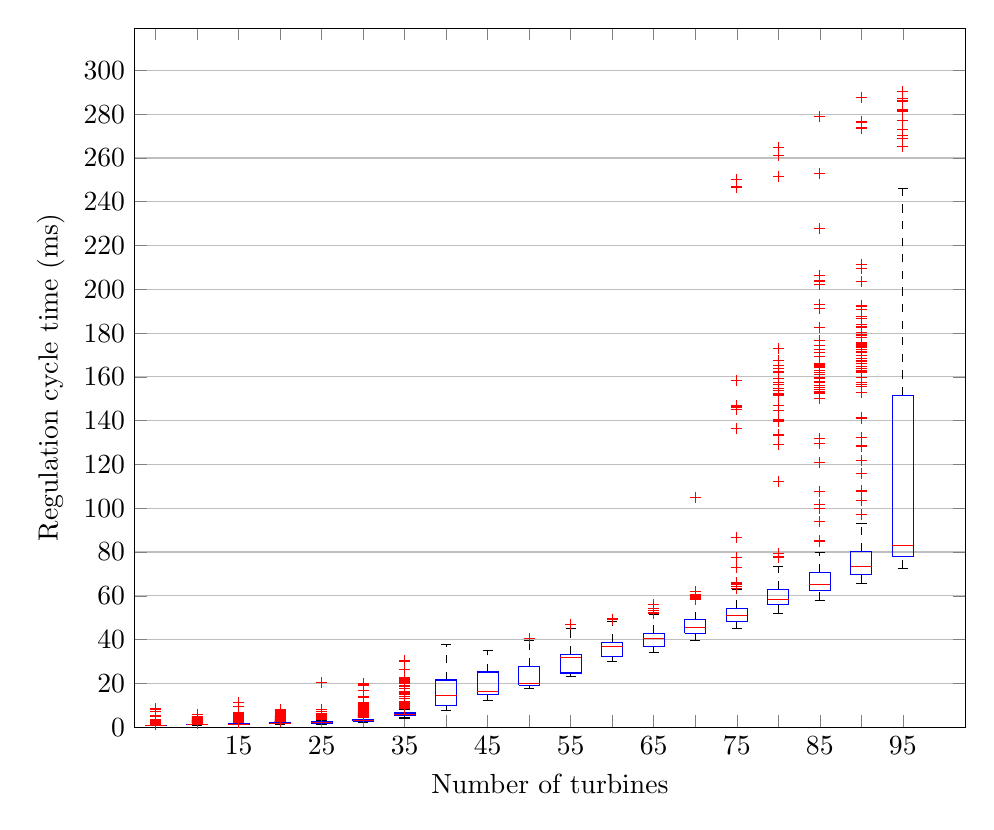
\begin{tikzpicture}

\begin{axis}[%
	width=\resultsPlotWidthScale\textwidth,
	xmin=0.5,
	xmax=20.5,
	xlabel=Number of turbines,
	ylabel=Regulation cycle time (ms),
	xtick={1, 2, 3, 4, 5, 6, 7, 8, 9, 10, 11, 12, 13, 14, 15, 16, 17, 18, 19},
	xticklabels={ , , 15, , 25, , 35, , 45, , 55, , 65, , 75, , 85, , 95},
	ymin=0,
%	ymax=300,
	ymajorgrids=true,
	yminorgrids=true,
	max space between ticks=17.5
]
\addplot [color=black,dashed,forget plot]
  table[row sep=crcr]{%
1	0.955499\\
1	1.156637\\
};
\addplot [color=black,dashed,forget plot]
  table[row sep=crcr]{%
2	1.370008\\
2	1.786582\\
};
\addplot [color=black,dashed,forget plot]
  table[row sep=crcr]{%
3	1.673373\\
3	2.174249\\
};
\addplot [color=black,dashed,forget plot]
  table[row sep=crcr]{%
4	1.958627\\
4	2.487973\\
};
\addplot [color=black,dashed,forget plot]
  table[row sep=crcr]{%
5	2.424964\\
5	3.23762\\
};
\addplot [color=black,dashed,forget plot]
  table[row sep=crcr]{%
6	3.359207\\
6	4.343135\\
};
\addplot [color=black,dashed,forget plot]
  table[row sep=crcr]{%
7	6.472311\\
7	8.243171\\
};
\addplot [color=black,dashed,forget plot]
  table[row sep=crcr]{%
8	21.564196\\
8	37.584364\\
};
\addplot [color=black,dashed,forget plot]
  table[row sep=crcr]{%
9	25.210282\\
9	34.938512\\
};
\addplot [color=black,dashed,forget plot]
  table[row sep=crcr]{%
10	27.678968\\
10	39.521324\\
};
\addplot [color=black,dashed,forget plot]
  table[row sep=crcr]{%
11	33.133063\\
11	45.066276\\
};
\addplot [color=black,dashed,forget plot]
  table[row sep=crcr]{%
12	38.659741\\
12	48.386618\\
};
\addplot [color=black,dashed,forget plot]
  table[row sep=crcr]{%
13	42.692349\\
13	51.64833\\
};
\addplot [color=black,dashed,forget plot]
  table[row sep=crcr]{%
14	48.995592\\
14	58.222076\\
};
\addplot [color=black,dashed,forget plot]
  table[row sep=crcr]{%
15	54.185768\\
15	62.996037\\
};
\addplot [color=black,dashed,forget plot]
  table[row sep=crcr]{%
16	62.88196\\
16	73.366361\\
};
\addplot [color=black,dashed,forget plot]
  table[row sep=crcr]{%
17	70.609667\\
17	79.750216\\
};
\addplot [color=black,dashed,forget plot]
  table[row sep=crcr]{%
18	80.203607\\
18	93.075175\\
};
\addplot [color=black,dashed,forget plot]
  table[row sep=crcr]{%
19	151.608592\\
19	246.076944\\
};
\addplot [color=black,dashed,forget plot]
  table[row sep=crcr]{%
1	0.691463\\
1	0.814662\\
};
\addplot [color=black,dashed,forget plot]
  table[row sep=crcr]{%
2	0.848749\\
2	1.088204\\
};
\addplot [color=black,dashed,forget plot]
  table[row sep=crcr]{%
3	1.082791\\
3	1.330567\\
};
\addplot [color=black,dashed,forget plot]
  table[row sep=crcr]{%
4	1.225531\\
4	1.59823\\
};
\addplot [color=black,dashed,forget plot]
  table[row sep=crcr]{%
5	1.440994\\
5	1.862917\\
};
\addplot [color=black,dashed,forget plot]
  table[row sep=crcr]{%
6	2.148756\\
6	2.694676\\
};
\addplot [color=black,dashed,forget plot]
  table[row sep=crcr]{%
7	4.178016\\
7	5.258074\\
};
\addplot [color=black,dashed,forget plot]
  table[row sep=crcr]{%
8	7.806459\\
8	9.763918\\
};
\addplot [color=black,dashed,forget plot]
  table[row sep=crcr]{%
9	12.116028\\
9	14.873879\\
};
\addplot [color=black,dashed,forget plot]
  table[row sep=crcr]{%
10	17.509834\\
10	19.152298\\
};
\addplot [color=black,dashed,forget plot]
  table[row sep=crcr]{%
11	23.186344\\
11	24.757905\\
};
\addplot [color=black,dashed,forget plot]
  table[row sep=crcr]{%
12	29.984252\\
12	32.129229\\
};
\addplot [color=black,dashed,forget plot]
  table[row sep=crcr]{%
13	33.953182\\
13	36.679471\\
};
\addplot [color=black,dashed,forget plot]
  table[row sep=crcr]{%
14	39.402015\\
14	42.832867\\
};
\addplot [color=black,dashed,forget plot]
  table[row sep=crcr]{%
15	45.162367\\
15	48.235799\\
};
\addplot [color=black,dashed,forget plot]
  table[row sep=crcr]{%
16	51.804628\\
16	55.840494\\
};
\addplot [color=black,dashed,forget plot]
  table[row sep=crcr]{%
17	57.925799\\
17	62.39761\\
};
\addplot [color=black,dashed,forget plot]
  table[row sep=crcr]{%
18	65.7218\\
18	69.72912\\
};
\addplot [color=black,dashed,forget plot]
  table[row sep=crcr]{%
19	72.589561\\
19	77.840082\\
};
\addplot [color=black,solid,forget plot]
  table[row sep=crcr]{%
0.875	1.156637\\
1.125	1.156637\\
};
\addplot [color=black,solid,forget plot]
  table[row sep=crcr]{%
1.875	1.786582\\
2.125	1.786582\\
};
\addplot [color=black,solid,forget plot]
  table[row sep=crcr]{%
2.875	2.174249\\
3.125	2.174249\\
};
\addplot [color=black,solid,forget plot]
  table[row sep=crcr]{%
3.875	2.487973\\
4.125	2.487973\\
};
\addplot [color=black,solid,forget plot]
  table[row sep=crcr]{%
4.875	3.23762\\
5.125	3.23762\\
};
\addplot [color=black,solid,forget plot]
  table[row sep=crcr]{%
5.875	4.343135\\
6.125	4.343135\\
};
\addplot [color=black,solid,forget plot]
  table[row sep=crcr]{%
6.875	8.243171\\
7.125	8.243171\\
};
\addplot [color=black,solid,forget plot]
  table[row sep=crcr]{%
7.875	37.584364\\
8.125	37.584364\\
};
\addplot [color=black,solid,forget plot]
  table[row sep=crcr]{%
8.875	34.938512\\
9.125	34.938512\\
};
\addplot [color=black,solid,forget plot]
  table[row sep=crcr]{%
9.875	39.521324\\
10.125	39.521324\\
};
\addplot [color=black,solid,forget plot]
  table[row sep=crcr]{%
10.875	45.066276\\
11.125	45.066276\\
};
\addplot [color=black,solid,forget plot]
  table[row sep=crcr]{%
11.875	48.386618\\
12.125	48.386618\\
};
\addplot [color=black,solid,forget plot]
  table[row sep=crcr]{%
12.875	51.64833\\
13.125	51.64833\\
};
\addplot [color=black,solid,forget plot]
  table[row sep=crcr]{%
13.875	58.222076\\
14.125	58.222076\\
};
\addplot [color=black,solid,forget plot]
  table[row sep=crcr]{%
14.875	62.996037\\
15.125	62.996037\\
};
\addplot [color=black,solid,forget plot]
  table[row sep=crcr]{%
15.875	73.366361\\
16.125	73.366361\\
};
\addplot [color=black,solid,forget plot]
  table[row sep=crcr]{%
16.875	79.750216\\
17.125	79.750216\\
};
\addplot [color=black,solid,forget plot]
  table[row sep=crcr]{%
17.875	93.075175\\
18.125	93.075175\\
};
\addplot [color=black,solid,forget plot]
  table[row sep=crcr]{%
18.875	246.076944\\
19.125	246.076944\\
};
\addplot [color=black,solid,forget plot]
  table[row sep=crcr]{%
0.875	0.691463\\
1.125	0.691463\\
};
\addplot [color=black,solid,forget plot]
  table[row sep=crcr]{%
1.875	0.848749\\
2.125	0.848749\\
};
\addplot [color=black,solid,forget plot]
  table[row sep=crcr]{%
2.875	1.082791\\
3.125	1.082791\\
};
\addplot [color=black,solid,forget plot]
  table[row sep=crcr]{%
3.875	1.225531\\
4.125	1.225531\\
};
\addplot [color=black,solid,forget plot]
  table[row sep=crcr]{%
4.875	1.440994\\
5.125	1.440994\\
};
\addplot [color=black,solid,forget plot]
  table[row sep=crcr]{%
5.875	2.148756\\
6.125	2.148756\\
};
\addplot [color=black,solid,forget plot]
  table[row sep=crcr]{%
6.875	4.178016\\
7.125	4.178016\\
};
\addplot [color=black,solid,forget plot]
  table[row sep=crcr]{%
7.875	7.806459\\
8.125	7.806459\\
};
\addplot [color=black,solid,forget plot]
  table[row sep=crcr]{%
8.875	12.116028\\
9.125	12.116028\\
};
\addplot [color=black,solid,forget plot]
  table[row sep=crcr]{%
9.875	17.509834\\
10.125	17.509834\\
};
\addplot [color=black,solid,forget plot]
  table[row sep=crcr]{%
10.875	23.186344\\
11.125	23.186344\\
};
\addplot [color=black,solid,forget plot]
  table[row sep=crcr]{%
11.875	29.984252\\
12.125	29.984252\\
};
\addplot [color=black,solid,forget plot]
  table[row sep=crcr]{%
12.875	33.953182\\
13.125	33.953182\\
};
\addplot [color=black,solid,forget plot]
  table[row sep=crcr]{%
13.875	39.402015\\
14.125	39.402015\\
};
\addplot [color=black,solid,forget plot]
  table[row sep=crcr]{%
14.875	45.162367\\
15.125	45.162367\\
};
\addplot [color=black,solid,forget plot]
  table[row sep=crcr]{%
15.875	51.804628\\
16.125	51.804628\\
};
\addplot [color=black,solid,forget plot]
  table[row sep=crcr]{%
16.875	57.925799\\
17.125	57.925799\\
};
\addplot [color=black,solid,forget plot]
  table[row sep=crcr]{%
17.875	65.7218\\
18.125	65.7218\\
};
\addplot [color=black,solid,forget plot]
  table[row sep=crcr]{%
18.875	72.589561\\
19.125	72.589561\\
};
\addplot [color=blue,solid,forget plot]
  table[row sep=crcr]{%
0.75	0.814662\\
0.75	0.955499\\
1.25	0.955499\\
1.25	0.814662\\
0.75	0.814662\\
};
\addplot [color=blue,solid,forget plot]
  table[row sep=crcr]{%
1.75	1.088204\\
1.75	1.370008\\
2.25	1.370008\\
2.25	1.088204\\
1.75	1.088204\\
};
\addplot [color=blue,solid,forget plot]
  table[row sep=crcr]{%
2.75	1.330567\\
2.75	1.673373\\
3.25	1.673373\\
3.25	1.330567\\
2.75	1.330567\\
};
\addplot [color=blue,solid,forget plot]
  table[row sep=crcr]{%
3.75	1.59823\\
3.75	1.958627\\
4.25	1.958627\\
4.25	1.59823\\
3.75	1.59823\\
};
\addplot [color=blue,solid,forget plot]
  table[row sep=crcr]{%
4.75	1.862917\\
4.75	2.424964\\
5.25	2.424964\\
5.25	1.862917\\
4.75	1.862917\\
};
\addplot [color=blue,solid,forget plot]
  table[row sep=crcr]{%
5.75	2.694676\\
5.75	3.359207\\
6.25	3.359207\\
6.25	2.694676\\
5.75	2.694676\\
};
\addplot [color=blue,solid,forget plot]
  table[row sep=crcr]{%
6.75	5.258074\\
6.75	6.472311\\
7.25	6.472311\\
7.25	5.258074\\
6.75	5.258074\\
};
\addplot [color=blue,solid,forget plot]
  table[row sep=crcr]{%
7.75	9.763918\\
7.75	21.564196\\
8.25	21.564196\\
8.25	9.763918\\
7.75	9.763918\\
};
\addplot [color=blue,solid,forget plot]
  table[row sep=crcr]{%
8.75	14.873879\\
8.75	25.210282\\
9.25	25.210282\\
9.25	14.873879\\
8.75	14.873879\\
};
\addplot [color=blue,solid,forget plot]
  table[row sep=crcr]{%
9.75	19.152298\\
9.75	27.678968\\
10.25	27.678968\\
10.25	19.152298\\
9.75	19.152298\\
};
\addplot [color=blue,solid,forget plot]
  table[row sep=crcr]{%
10.75	24.757905\\
10.75	33.133063\\
11.25	33.133063\\
11.25	24.757905\\
10.75	24.757905\\
};
\addplot [color=blue,solid,forget plot]
  table[row sep=crcr]{%
11.75	32.129229\\
11.75	38.659741\\
12.25	38.659741\\
12.25	32.129229\\
11.75	32.129229\\
};
\addplot [color=blue,solid,forget plot]
  table[row sep=crcr]{%
12.75	36.679471\\
12.75	42.692349\\
13.25	42.692349\\
13.25	36.679471\\
12.75	36.679471\\
};
\addplot [color=blue,solid,forget plot]
  table[row sep=crcr]{%
13.75	42.832867\\
13.75	48.995592\\
14.25	48.995592\\
14.25	42.832867\\
13.75	42.832867\\
};
\addplot [color=blue,solid,forget plot]
  table[row sep=crcr]{%
14.75	48.235799\\
14.75	54.185768\\
15.25	54.185768\\
15.25	48.235799\\
14.75	48.235799\\
};
\addplot [color=blue,solid,forget plot]
  table[row sep=crcr]{%
15.75	55.840494\\
15.75	62.88196\\
16.25	62.88196\\
16.25	55.840494\\
15.75	55.840494\\
};
\addplot [color=blue,solid,forget plot]
  table[row sep=crcr]{%
16.75	62.39761\\
16.75	70.609667\\
17.25	70.609667\\
17.25	62.39761\\
16.75	62.39761\\
};
\addplot [color=blue,solid,forget plot]
  table[row sep=crcr]{%
17.75	69.72912\\
17.75	80.203607\\
18.25	80.203607\\
18.25	69.72912\\
17.75	69.72912\\
};
\addplot [color=blue,solid,forget plot]
  table[row sep=crcr]{%
18.75	77.840082\\
18.75	151.608592\\
19.25	151.608592\\
19.25	77.840082\\
18.75	77.840082\\
};
\addplot [color=red,solid,forget plot]
  table[row sep=crcr]{%
0.75	0.874626\\
1.25	0.874626\\
};
\addplot [color=red,solid,forget plot]
  table[row sep=crcr]{%
1.75	1.1775345\\
2.25	1.1775345\\
};
\addplot [color=red,solid,forget plot]
  table[row sep=crcr]{%
2.75	1.4201575\\
3.25	1.4201575\\
};
\addplot [color=red,solid,forget plot]
  table[row sep=crcr]{%
3.75	1.716257\\
4.25	1.716257\\
};
\addplot [color=red,solid,forget plot]
  table[row sep=crcr]{%
4.75	1.9973935\\
5.25	1.9973935\\
};
\addplot [color=red,solid,forget plot]
  table[row sep=crcr]{%
5.75	2.903549\\
6.25	2.903549\\
};
\addplot [color=red,solid,forget plot]
  table[row sep=crcr]{%
6.75	5.5932275\\
7.25	5.5932275\\
};
\addplot [color=red,solid,forget plot]
  table[row sep=crcr]{%
7.75	14.5812775\\
8.25	14.5812775\\
};
\addplot [color=red,solid,forget plot]
  table[row sep=crcr]{%
8.75	16.4337625\\
9.25	16.4337625\\
};
\addplot [color=red,solid,forget plot]
  table[row sep=crcr]{%
9.75	20.091426\\
10.25	20.091426\\
};
\addplot [color=red,solid,forget plot]
  table[row sep=crcr]{%
10.75	31.692363\\
11.25	31.692363\\
};
\addplot [color=red,solid,forget plot]
  table[row sep=crcr]{%
11.75	36.8004425\\
12.25	36.8004425\\
};
\addplot [color=red,solid,forget plot]
  table[row sep=crcr]{%
12.75	40.4086135\\
13.25	40.4086135\\
};
\addplot [color=red,solid,forget plot]
  table[row sep=crcr]{%
13.75	45.333356\\
14.25	45.333356\\
};
\addplot [color=red,solid,forget plot]
  table[row sep=crcr]{%
14.75	50.8482875\\
15.25	50.8482875\\
};
\addplot [color=red,solid,forget plot]
  table[row sep=crcr]{%
15.75	58.49032\\
16.25	58.49032\\
};
\addplot [color=red,solid,forget plot]
  table[row sep=crcr]{%
16.75	65.293539\\
17.25	65.293539\\
};
\addplot [color=red,solid,forget plot]
  table[row sep=crcr]{%
17.75	73.479706\\
18.25	73.479706\\
};
\addplot [color=red,solid,forget plot]
  table[row sep=crcr]{%
18.75	82.948313\\
19.25	82.948313\\
};
\addplot [color=blue,only marks,mark=+,mark options={solid,draw=red},forget plot]
  table[row sep=crcr]{%
1	1.176103\\
1	1.178509\\
1	1.193344\\
1	1.20704\\
1	1.214954\\
1	1.221493\\
1	1.245021\\
1	1.316445\\
1	1.327208\\
1	1.524131\\
1	1.524274\\
1	1.543741\\
1	1.902597\\
1	2.169802\\
1	2.307744\\
1	2.476555\\
1	2.709384\\
1	2.981451\\
1	3.140805\\
1	3.283617\\
1	4.963499\\
1	5.363371\\
1	7.190786\\
1	8.30093\\
};
\addplot [color=blue,only marks,mark=+,mark options={solid,draw=red},forget plot]
  table[row sep=crcr]{%
2	1.793523\\
2	1.845619\\
2	1.848076\\
2	1.933673\\
2	1.99282\\
2	2.051408\\
2	2.120934\\
2	2.151493\\
2	2.249679\\
2	2.262758\\
2	2.300418\\
2	2.368791\\
2	2.401617\\
2	2.481835\\
2	2.53602\\
2	2.548682\\
2	2.576888\\
2	2.597632\\
2	2.677461\\
2	2.723364\\
2	2.740618\\
2	2.774466\\
2	2.867248\\
2	2.899936\\
2	2.944661\\
2	2.965056\\
2	2.96526\\
2	2.981629\\
2	3.089347\\
2	3.131373\\
2	3.180755\\
2	3.306036\\
2	3.332826\\
2	3.449926\\
2	3.489132\\
2	3.672439\\
2	3.706892\\
2	3.749078\\
2	3.877362\\
2	4.023028\\
2	4.389004\\
2	4.398121\\
2	4.401876\\
2	4.678904\\
2	4.779742\\
2	4.918733\\
2	5.075662\\
2	5.601809\\
};
\addplot [color=blue,only marks,mark=+,mark options={solid,draw=red},forget plot]
  table[row sep=crcr]{%
3	2.192261\\
3	2.222847\\
3	2.223433\\
3	2.239635\\
3	2.245748\\
3	2.337855\\
3	2.564155\\
3	2.566424\\
3	2.568352\\
3	2.629852\\
3	2.652528\\
3	2.703118\\
3	2.733534\\
3	2.764757\\
3	2.783863\\
3	2.828118\\
3	2.846928\\
3	2.984215\\
3	3.051839\\
3	3.071094\\
3	3.081963\\
3	3.230031\\
3	3.352067\\
3	3.690988\\
3	3.70011\\
3	3.71423\\
3	4.081016\\
3	4.251259\\
3	4.299668\\
3	4.317077\\
3	4.378226\\
3	4.655414\\
3	4.800068\\
3	5.335757\\
3	5.455589\\
3	5.596238\\
3	5.710081\\
3	5.790715\\
3	6.364993\\
3	6.679123\\
3	9.543143\\
3	11.395216\\
};
\addplot [color=blue,only marks,mark=+,mark options={solid,draw=red},forget plot]
  table[row sep=crcr]{%
4	2.503863\\
4	2.506996\\
4	2.518698\\
4	2.519083\\
4	2.524849\\
4	2.538949\\
4	2.539779\\
4	2.543708\\
4	2.590436\\
4	2.612976\\
4	2.624723\\
4	2.639969\\
4	2.692657\\
4	2.701875\\
4	2.702706\\
4	2.776353\\
4	2.834106\\
4	2.874534\\
4	2.903889\\
4	2.921809\\
4	2.947651\\
4	3.016038\\
4	3.18633\\
4	3.256435\\
4	3.289407\\
4	3.470499\\
4	3.523172\\
4	3.573076\\
4	3.614098\\
4	3.621255\\
4	3.757607\\
4	3.911986\\
4	4.033259\\
4	4.073237\\
4	4.338524\\
4	4.399647\\
4	4.630443\\
4	4.664954\\
4	4.779427\\
4	4.906645\\
4	4.925404\\
4	5.040655\\
4	5.079302\\
4	5.373808\\
4	6.030455\\
4	6.328306\\
4	6.626284\\
4	6.999776\\
4	7.221142\\
4	7.451491\\
4	7.916905\\
};
\addplot [color=blue,only marks,mark=+,mark options={solid,draw=red},forget plot]
  table[row sep=crcr]{%
5	3.320071\\
5	3.377586\\
5	3.423061\\
5	3.427332\\
5	3.53449\\
5	3.546939\\
5	3.746197\\
5	3.765826\\
5	3.782267\\
5	3.787644\\
5	3.824862\\
5	3.893861\\
5	3.959252\\
5	4.037436\\
5	4.097061\\
5	4.125631\\
5	4.133696\\
5	4.138075\\
5	4.147994\\
5	4.176374\\
5	4.421668\\
5	4.513637\\
5	4.616056\\
5	4.635814\\
5	4.753148\\
5	5.167944\\
5	5.19975\\
5	5.420932\\
5	5.455067\\
5	5.665121\\
5	5.721665\\
5	5.83401\\
5	5.87468\\
5	5.89412\\
5	5.921696\\
5	6.057049\\
5	6.131888\\
5	6.296973\\
5	6.321923\\
5	6.343328\\
5	7.090603\\
5	8.26168\\
5	20.243534\\
};
\addplot [color=blue,only marks,mark=+,mark options={solid,draw=red},forget plot]
  table[row sep=crcr]{%
6	4.495225\\
6	4.498673\\
6	4.498827\\
6	4.563186\\
6	4.587355\\
6	4.754654\\
6	5.009052\\
6	5.021732\\
6	5.102506\\
6	5.158721\\
6	5.167734\\
6	5.198709\\
6	5.23857\\
6	5.3746\\
6	5.400768\\
6	5.471458\\
6	5.487853\\
6	5.732529\\
6	5.758585\\
6	5.785591\\
6	5.904012\\
6	6.088597\\
6	6.13559\\
6	6.338497\\
6	6.607769\\
6	6.707598\\
6	6.847774\\
6	6.863557\\
6	6.923896\\
6	6.932131\\
6	6.966114\\
6	7.246241\\
6	7.552089\\
6	7.637072\\
6	8.035988\\
6	8.318994\\
6	8.349444\\
6	8.519427\\
6	8.777099\\
6	9.338181\\
6	9.720935\\
6	9.898789\\
6	10.188432\\
6	10.358991\\
6	10.590425\\
6	11.26527\\
6	13.649585\\
6	13.917339\\
6	16.898115\\
6	19.216894\\
6	19.71008\\
};
\addplot [color=blue,only marks,mark=+,mark options={solid,draw=red},forget plot]
  table[row sep=crcr]{%
7	8.35779\\
7	8.415277\\
7	8.473364\\
7	8.504532\\
7	8.506126\\
7	8.519745\\
7	8.553583\\
7	8.5815\\
7	8.663745\\
7	8.678187\\
7	8.683617\\
7	8.78386\\
7	8.849726\\
7	8.950628\\
7	8.987027\\
7	8.992308\\
7	9.120563\\
7	9.207595\\
7	9.23472\\
7	9.345101\\
7	9.398249\\
7	9.423573\\
7	9.439464\\
7	9.486276\\
7	9.521467\\
7	9.580156\\
7	9.590542\\
7	9.629696\\
7	9.657168\\
7	9.679038\\
7	9.768644\\
7	9.773259\\
7	9.820831\\
7	9.965677\\
7	10.269888\\
7	10.302693\\
7	10.323261\\
7	10.420508\\
7	10.88144\\
7	10.912448\\
7	10.912924\\
7	10.922096\\
7	11.006882\\
7	11.222083\\
7	11.30686\\
7	11.547859\\
7	13.009371\\
7	14.092999\\
7	14.86172\\
7	15.293268\\
7	15.773637\\
7	16.071576\\
7	17.524366\\
7	18.635734\\
7	18.86347\\
7	18.884021\\
7	19.925684\\
7	20.211662\\
7	20.368998\\
7	20.490724\\
7	20.838327\\
7	20.957185\\
7	21.053338\\
7	21.479073\\
7	21.720464\\
7	21.952807\\
7	22.450527\\
7	26.466628\\
7	29.810133\\
7	29.924012\\
7	30.656609\\
};
\addplot [color=blue,only marks,mark=+,mark options={solid,draw=red},forget plot]
  table[row sep=crcr]{%
nan	nan\\
};
\addplot [color=blue,only marks,mark=+,mark options={solid,draw=red},forget plot]
  table[row sep=crcr]{%
nan	nan\\
};
\addplot [color=blue,only marks,mark=+,mark options={solid,draw=red},forget plot]
  table[row sep=crcr]{%
10	40.572149\\
};
\addplot [color=blue,only marks,mark=+,mark options={solid,draw=red},forget plot]
  table[row sep=crcr]{%
11	46.841843\\
};
\addplot [color=blue,only marks,mark=+,mark options={solid,draw=red},forget plot]
  table[row sep=crcr]{%
12	49.32547\\
12	49.39728\\
};
\addplot [color=blue,only marks,mark=+,mark options={solid,draw=red},forget plot]
  table[row sep=crcr]{%
13	51.734931\\
13	52.263042\\
13	52.479868\\
13	53.346653\\
13	53.380803\\
13	54.235959\\
13	56.218855\\
};
\addplot [color=blue,only marks,mark=+,mark options={solid,draw=red},forget plot]
  table[row sep=crcr]{%
14	58.24263\\
14	58.359494\\
14	58.779699\\
14	59.255721\\
14	59.797221\\
14	59.956779\\
14	59.989437\\
14	60.023581\\
14	60.358906\\
14	60.684411\\
14	61.858036\\
14	104.953184\\
};
\addplot [color=blue,only marks,mark=+,mark options={solid,draw=red},forget plot]
  table[row sep=crcr]{%
15	63.495834\\
15	64.370846\\
15	65.078212\\
15	65.674834\\
15	65.803883\\
15	65.835327\\
15	66.021914\\
15	66.103339\\
15	73.001122\\
15	77.636315\\
15	86.826142\\
15	136.487634\\
15	145.283402\\
15	146.099428\\
15	146.233285\\
15	146.323243\\
15	146.921872\\
15	158.423312\\
15	246.362832\\
15	246.722952\\
15	250.200229\\
};
\addplot [color=blue,only marks,mark=+,mark options={solid,draw=red},forget plot]
  table[row sep=crcr]{%
16	77.720929\\
16	79.177628\\
16	112.408851\\
16	128.969515\\
16	133.462981\\
16	139.858548\\
16	140.725977\\
16	144.612062\\
16	146.817379\\
16	151.383076\\
16	151.881108\\
16	151.922485\\
16	152.242982\\
16	153.688064\\
16	154.509165\\
16	156.475983\\
16	157.507242\\
16	159.324566\\
16	162.256717\\
16	164.015403\\
16	165.32339\\
16	167.323423\\
16	172.786236\\
16	251.349021\\
16	261.289044\\
16	264.827819\\
};
\addplot [color=blue,only marks,mark=+,mark options={solid,draw=red},forget plot]
  table[row sep=crcr]{%
17	85.033259\\
17	85.168934\\
17	93.984073\\
17	99.985429\\
17	101.754141\\
17	107.502865\\
17	120.708505\\
17	129.533025\\
17	131.685524\\
17	150.07707\\
17	152.531279\\
17	152.848707\\
17	153.515564\\
17	154.184764\\
17	154.425517\\
17	155.223244\\
17	155.325952\\
17	156.040595\\
17	157.51096\\
17	157.745791\\
17	157.763823\\
17	157.78978\\
17	159.313071\\
17	159.792905\\
17	161.075164\\
17	161.182074\\
17	161.201118\\
17	162.147412\\
17	163.084965\\
17	164.144737\\
17	164.432633\\
17	164.531559\\
17	165.276971\\
17	165.915944\\
17	166.24057\\
17	169.122972\\
17	170.956902\\
17	172.574969\\
17	174.203491\\
17	174.230232\\
17	176.682499\\
17	182.438894\\
17	191.366639\\
17	192.967176\\
17	202.370675\\
17	203.807066\\
17	206.229644\\
17	227.845875\\
17	252.720361\\
17	278.866888\\
};
\addplot [color=blue,only marks,mark=+,mark options={solid,draw=red},forget plot]
  table[row sep=crcr]{%
18	97.320739\\
18	103.607594\\
18	107.896473\\
18	116.060945\\
18	121.809576\\
18	128.452211\\
18	132.177856\\
18	141.230189\\
18	152.923783\\
18	155.730984\\
18	156.691553\\
18	157.523825\\
18	159.835414\\
18	159.897403\\
18	161.962464\\
18	162.510937\\
18	162.565594\\
18	163.007536\\
18	163.988911\\
18	164.705291\\
18	165.959133\\
18	167.195639\\
18	167.26318\\
18	167.489415\\
18	167.573509\\
18	168.458682\\
18	169.70467\\
18	171.087881\\
18	171.523672\\
18	171.531448\\
18	171.659207\\
18	172.561978\\
18	172.716008\\
18	173.315331\\
18	173.869469\\
18	174.119127\\
18	174.807872\\
18	175.47089\\
18	178.054177\\
18	178.925643\\
18	179.325541\\
18	180.261783\\
18	182.703061\\
18	183.168246\\
18	183.804264\\
18	186.546645\\
18	187.398376\\
18	190.73619\\
18	192.117568\\
18	192.334748\\
18	192.687149\\
18	203.621105\\
18	209.714732\\
18	211.529157\\
18	273.591922\\
18	274.074762\\
18	276.443283\\
18	287.542878\\
};
\addplot [color=blue,only marks,mark=+,mark options={solid,draw=red},forget plot]
  table[row sep=crcr]{%
19	265.296814\\
19	268.749173\\
19	270.245766\\
19	273.069504\\
19	277.122711\\
19	281.054363\\
19	281.926684\\
19	282.148412\\
19	285.594887\\
19	286.16293\\
19	287.331069\\
19	290.243704\\
};
\node[above, align=center, inner sep=0mm, text=black]
at (axis cs:9.13684210526316,-12,0) {1};
\node[above, align=center, inner sep=0mm, text=black]
at (axis cs:27.4105263157895,-12,0) {2};
\node[above, align=center, inner sep=0mm, text=black]
at (axis cs:45.6842105263158,-12,0) {3};
\node[above, align=center, inner sep=0mm, text=black]
at (axis cs:63.9578947368421,-12,0) {4};
\node[above, align=center, inner sep=0mm, text=black]
at (axis cs:82.2315789473684,-12,0) {5};
\node[above, align=center, inner sep=0mm, text=black]
at (axis cs:100.505263157895,-12,0) {6};
\node[above, align=center, inner sep=0mm, text=black]
at (axis cs:118.778947368421,-12,0) {7};
\node[above, align=center, inner sep=0mm, text=black]
at (axis cs:137.052631578947,-12,0) {8};
\node[above, align=center, inner sep=0mm, text=black]
at (axis cs:155.326315789474,-12,0) {9};
\node[above, align=center, inner sep=0mm, text=black]
at (axis cs:173.6,-12,0) {10};
\node[above, align=center, inner sep=0mm, text=black]
at (axis cs:191.873684210526,-12,0) {11};
\node[above, align=center, inner sep=0mm, text=black]
at (axis cs:210.147368421053,-12,0) {12};
\node[above, align=center, inner sep=0mm, text=black]
at (axis cs:228.421052631579,-12,0) {13};
\node[above, align=center, inner sep=0mm, text=black]
at (axis cs:246.694736842105,-12,0) {14};
\node[above, align=center, inner sep=0mm, text=black]
at (axis cs:264.968421052632,-12,0) {15};
\node[above, align=center, inner sep=0mm, text=black]
at (axis cs:283.242105263158,-12,0) {16};
\node[above, align=center, inner sep=0mm, text=black]
at (axis cs:301.515789473684,-12,0) {17};
\node[above, align=center, inner sep=0mm, text=black]
at (axis cs:319.789473684211,-12,0) {18};
\node[above, align=center, inner sep=0mm, text=black]
at (axis cs:338.063157894737,-12,0) {19};
\end{axis}
\end{tikzpicture}%
	
	\caption{Centralized solution variable number of turbines}
	\label{fig:exp:cen:turbines}
\end{figure}

\Cref{fig:exp:cen:turbines} shows how the number of turbines influence the regulation cycle time of the centralized solution.
For every number of turbines 450 data points have been sampled. The reason for the limited amount of samples is that when running the experiment with 95 turbines the test setup is reaching it's limits. Data transfer speeds of up to 75 Mbit/s was observed. Since the maximum theoretical data transfer speed of the test setup is 100 Mbit/s it is reasonable to assume that a number of packages have been lost due to congestion. Thus, the experiment for 95 turbines only managed to log 450 data samples within the given experiment time. In order to create a boxplot with comparable values the sample set for each number of turbines was reduced to the 450 first points.
The limited amount of data samples account for the "holes" between outlier values. With more data samples these holes would be filled such that outliers are more evenly distributed from the top whisker to the most extreme outlier.

The median values from 5 to 30 turbines is increasing slightly. From 35 turbines and onward the median is linearly increasing.
From 75 turbines onward the outliers take on increasingly extreme values, which is when the test setup starts to be unable to handle the number of packages sent in the network. Results from 75 turbines and onward should be disregarded.

\subsection{Discussion}
The test results from the centralized solution presented in \cref{fig:exp:cen:turbines} shows how adding turbines increases the regulation cycle time. From 5 to 30 turbines the regulation time of the centralized solution increase slowly. After 35 turbines the increase in regulation cycle time becomes steeper. For every 15 turbines added the regulation cycle time increases with approximately $25 ms$. The relation between regulation cycle time and the number of turbines is caused by the direct impact the number of turbines have on the regulation cycle. The Park Pilot of the centralized solution must use additional time on querying each added turbine as well as wait for their individual reply before performing the regulation algorithm. Thus the scalability of the centralized solution is linear with a factor of approximately $25 / 15 = 1.667$ ms added regulation cycle time per added turbine.
The outliers of \cref{fig:exp:cen:turbines} is distributed fairly close around the medains from 5 to 70 turbines. From 75 turbines on the outliers quadruple in regulation cycle time which is a sign that the test setup has reached it's limits. The heavily increased regulation cycle time for the outliers is a result of lost or delayed network packages forcing the Park Pilot to wait for a retransmission of turbine state before the regulation cycle can be completed.

\subsubsection{Comparison of the decentralized solution and the centralized solution}
\label{sec:comp:decentralizedVScentralized}
The decentralized solution and the centralized solution is built with a very different architecture. This is reflected in the difference in the way the two solutions scale with the number of turbines.

\cref{fig:exp:cenVSDecen} shows the medians of \cref{fig:exp:decen:turbines,fig:exp:cen:turbines} where data that has been disregarded previously has been removed. Thus, the maximum number of turbines in \cref{fig:exp:cenVSDecen} is 70. 

\begin{figure}[h!]
	\centering
		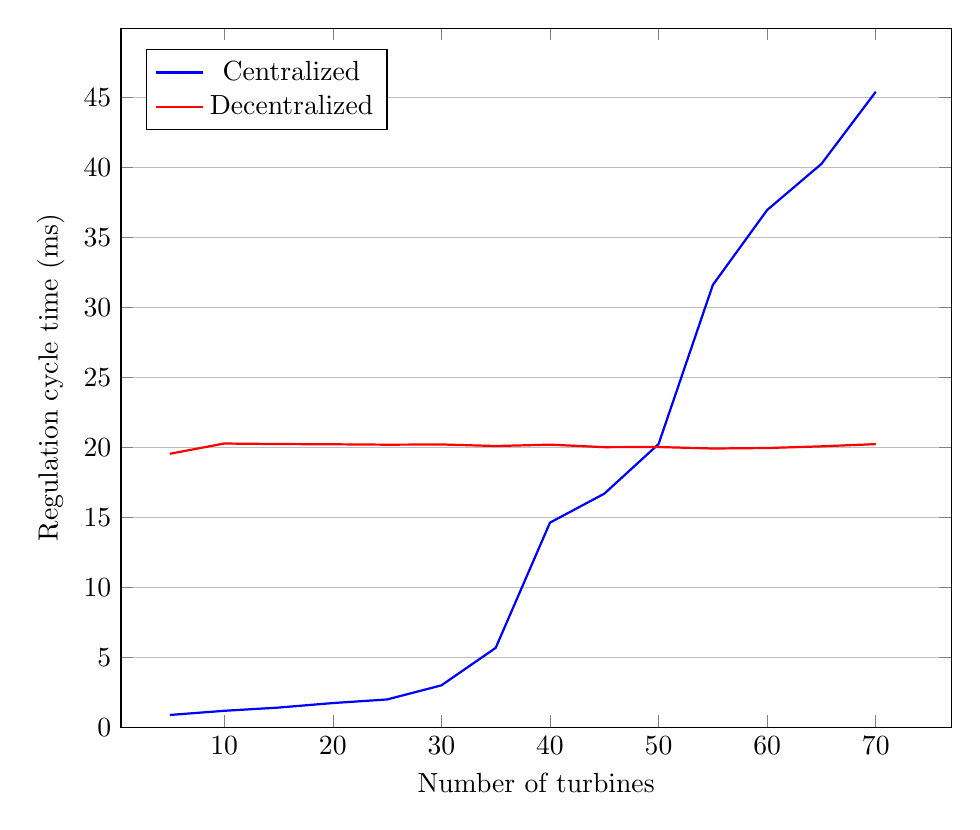
\begin{tikzpicture}
	
	\begin{axis}[%
	width=\resultsPlotWidthScale\textwidth,
	xmin=0.5,
%	xmax=20.5,
	xlabel=Number of turbines,
	ylabel=Regulation cycle time (ms),
%	xtick={1, 2, 3, 4, 5, 6, 7, 8, 9, 10, 11, 12, 13, 14, 15, 16, 17, 18, 19},
%	xticklabels={ 5, , 15, , 25, , 35, , 45, , 55, , 65, , 75, , 85, , 95},
	ymin=0,
	%	ymax=300,
	ymajorgrids=true,
%	yminorgrids=true,
%	max space between ticks=17.5,
	legend entries={Centralized,Decentralized},
	legend style={
		legend pos= north west,
	}
	]
	
	\addplot[thick, blue] coordinates {
		(5 ,0.871522)
		(10 ,1.168815)
		(15 ,1.398871)
		(20 ,1.722236)
		(25 ,1.978881)
		(30 ,2.985681)
		(35 ,5.662268)
		(40 ,14.607313)
		(45 ,16.673738)
		(50 ,20.220936)
		(55 ,31.587407)
		(60 ,36.93711)
		(65 ,40.231022)
		(70 ,45.380062)
%		(75 ,51.425649)
%		(80 ,58.196177)
%		(85 ,64.70376)
%		(90 ,73.715686)
%		(95 ,82.961949)
	};
	
	\addplot[thick, red] coordinates {
		(5 ,19.526002) 
		(10 ,20.257002)
		(15 ,20.221001)
		(20 ,20.203002)
		(25 ,20.174001)
		(30 ,20.190001)
		(35 ,20.079)
		(40 ,20.176)
		(45 ,19.998)
		(50 ,20.008)
		(55 ,19.902002)
		(60 ,19.937001)
		(65 ,20.056)
		(70 ,20.215)
%		(75 ,19.920001)
%		(80 ,20.129002)
%		(85 ,20.189001)
%		(90 ,20.902001)
%		(95 ,27.909001)
%		(100 ,43.314001)
	};
	\end{axis}
	\end{tikzpicture}	
	\caption{The centralized solution's median values compared with the decentralized solution's median values}
	\label{fig:exp:cenVSDecen}
\end{figure}

Looking at \cref{fig:exp:cenVSDecen} we see that the centralized and decentralized solutions scale very differently.
The decentralized solution scales constant with number of turbines from 5 to 70 turbines. The centralized solution scales linearly with the number of turbines from 5 to 30 turbines and from 30 to 70 turbines with a steeper slope. With the test setup used and a sleep time in the decentralized solution's regulation cycle at 20 ms the centralized solution scales better than the decentralized solution from 5 to 50 turbines. The decentralized solution scales better than the centralized solution from 50 to 70 turbines.
If the sleep time of the regulation cycle in the decentralized solution is lowered to for instance 10 ms the decentralized solution would scale better than the centralized solution from 38 turbines on. Lowering the sleep time of the regulation cycle in the decentralized solution will make the chance of cache reads increase as illustrated in \cref{fig:exp:decen:sleep-cache}.

One of the reasons for the constant scalability of the decentralized solution is the use of multicast in opposition to the centralized solution which uses unicast.
Using multicast the network communication is decreased compared to unicast, thus the network is less congested in the decentralized solution compared to the centralized solution.

Adding a turbine to the decentralized solution adds an extra turbine state to read into the setpoint calculation in the regulation algorithm, thus adding network traffic to the system.

As the test setup imposes limits on the number of turbines that can be simulated it is not possible to say anything concrete about how the scalability of the centralized and decentralized solution will be for any number of turbines higher than 70.
A qualified guess about the scalability can be provided though. The scalability of the centralized solution is expected to keep scaling linearly with the number of turbines. The decentralized solution will keep scaling with the number of turbines but as the number of turbines increase so will the number of cache reads. If the number of cache reads increases this will be reflected in the regulation cycle time. Thus, the scalability of the decentralized solution will not keep scaling at a constant level but the impact of increased cache reads remains to be further investigated.



\FloatBarrier

%The scalability of the centralized solution is linear with a factor of approximately $1.667$ ms added to regulation cycle time per turbine added to the system.
%The scalability of the decentralized solution, as described in \cref{sec:disc:turbinesVScycletime}, is small enough that it is indistinguishable from other factors in our test data and therefore we cannot calculate it. Thus the scalability of the decentralized solution is close to constant. This great improvement in scalability comes with a trade off in terms of cache reads. Adding additional turbines to the decentralized solution the number of cache reads increases with a factor of $0.033$ extra cache reads per added turbine which is still an improvement compared to the scale factor of the centralized solution. Arguably comparing the scalability of the number of cache reads in the decentralized solution with the scalability of the regulation cycle in the centralized solution is not a viable way to compare the scalability of the two solutions, but comparing the scalability of the regulation cycle of both solutions will not be a fair comparison either since the improvements in scalability of the decentralized solution comes at the price of increased numbers of cache reads.

\subsubsection{Comparison of the decentralized solution and the current Siemens system}
This section address the \ref{PS:Q:Scalability} problem of \cref{sec:problemStatement}.
Comparing the decentralized solution and the current Siemens system directly is impossible given the differences in environment and architecture. Introducing a centralized solution is an attempt to bridge this gap. By comparing the decentralized solution to the centralized solution and measuring the improvements/demotions we can transfer these measures to the current Siemens system and an imagined decentralized version of the current Siemens system.

Looking at \cref{sec:comp:decentralizedVScentralized} there is an advantage in scalability when running a decentralized solution compared to a centralized. This is underlined by the improvement in regulation cycle time of the decentralized solution compared to the centralized solution. The improvement of the scalability of the regulation cycle time comes at the price of the chance that the regulation may be performed on cached data.

Decentralizing the current Siemens system will enable improvements on other areas than regulation cycle time. By removing the centralized Park Pilots and the Wind Power Supervisor of the current Siemens solution the regulation of turbines, data storage and external communication of these must be decentralized and placed in the turbines themselves. This requires the use of software components that are able to handle regulation of turbines, data storage and external communication in a fashion such that if a turbine failure occurs other turbines can increase production to make up for the missing power production, provide access to the data collected on the failing turbine and handle external communication the failing turbine may have been handling. This increases the availability of the wind farm compared to the current Siemens system.




